% Created by tikzDevice version 0.7.0 on 2014-06-17 20:11:16
% !TEX encoding = UTF-8 Unicode
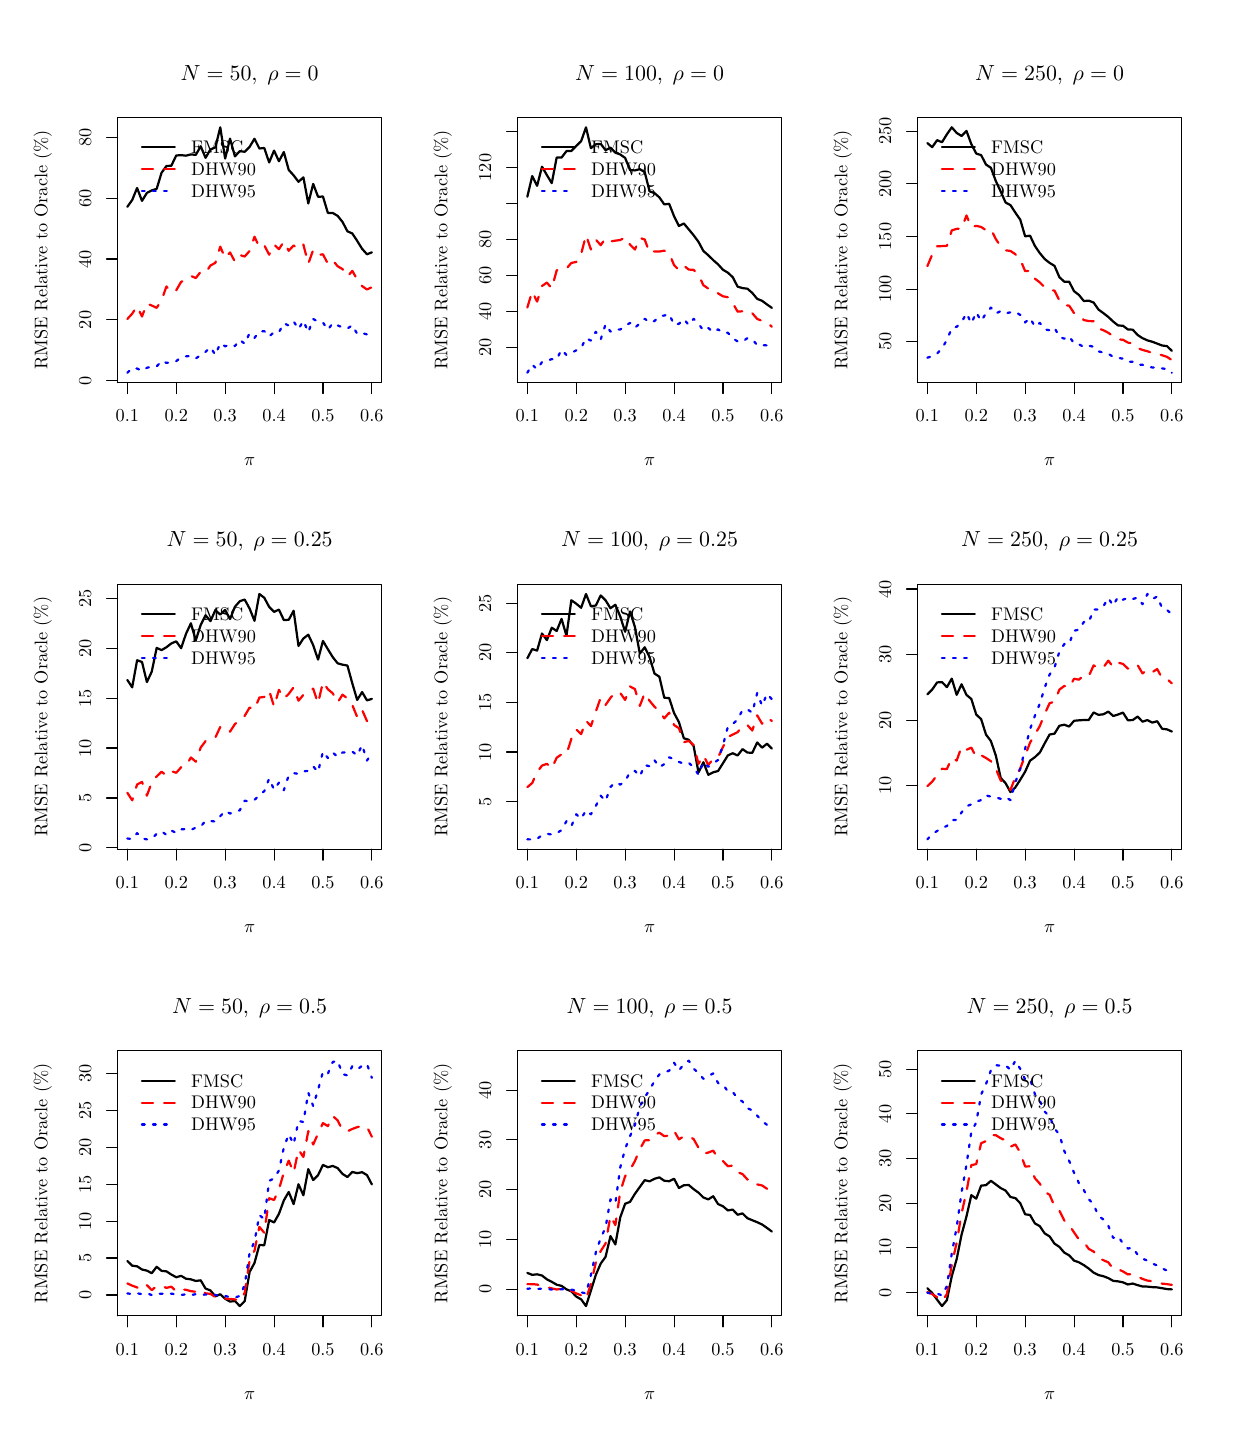
\begin{tikzpicture}[x=1pt,y=1pt]
\definecolor[named]{fillColor}{rgb}{1.00,1.00,1.00}
\path[use as bounding box,fill=fillColor,fill opacity=0.00] (0,0) rectangle (433.62,505.89);
\begin{scope}
\path[clip] ( 32.47,377.65) rectangle (127.91,473.42);
\definecolor[named]{drawColor}{rgb}{0.00,0.00,0.00}

\path[draw=drawColor,line width= 0.8pt,line join=round,line cap=round] ( 36.01,441.15) --
	( 37.77,443.61) --
	( 39.54,447.96) --
	( 41.31,443.30) --
	( 43.08,446.17) --
	( 44.84,447.09) --
	( 46.61,447.63) --
	( 48.38,453.47) --
	( 50.15,455.90) --
	( 51.91,456.00) --
	( 53.68,459.70) --
	( 55.45,459.82) --
	( 57.21,459.63) --
	( 58.98,460.10) --
	( 60.75,459.91) --
	( 62.52,463.04) --
	( 64.28,458.86) --
	( 66.05,461.90) --
	( 67.82,462.60) --
	( 69.59,469.87) --
	( 71.35,458.59) --
	( 73.12,465.79) --
	( 74.89,459.38) --
	( 76.66,461.27) --
	( 78.42,461.04) --
	( 80.19,462.81) --
	( 81.96,465.75) --
	( 83.72,462.23) --
	( 85.49,462.41) --
	( 87.26,457.19) --
	( 89.03,461.47) --
	( 90.79,457.62) --
	( 92.56,460.94) --
	( 94.33,454.48) --
	( 96.10,452.52) --
	( 97.86,450.19) --
	( 99.63,451.80) --
	(101.40,442.37) --
	(103.17,449.44) --
	(104.93,444.77) --
	(106.70,444.87) --
	(108.47,438.95) --
	(110.23,438.94) --
	(112.00,437.88) --
	(113.77,435.68) --
	(115.54,432.30) --
	(117.30,431.52) --
	(119.07,428.83) --
	(120.84,425.98) --
	(122.61,424.00) --
	(124.37,424.70);
\end{scope}
\begin{scope}
\path[clip] (  0.00,  0.00) rectangle (433.62,505.89);
\definecolor[named]{drawColor}{rgb}{0.00,0.00,0.00}

\path[draw=drawColor,line width= 0.4pt,line join=round,line cap=round] ( 36.01,377.65) -- (124.37,377.65);

\path[draw=drawColor,line width= 0.4pt,line join=round,line cap=round] ( 36.01,377.65) -- ( 36.01,373.69);

\path[draw=drawColor,line width= 0.4pt,line join=round,line cap=round] ( 53.68,377.65) -- ( 53.68,373.69);

\path[draw=drawColor,line width= 0.4pt,line join=round,line cap=round] ( 71.35,377.65) -- ( 71.35,373.69);

\path[draw=drawColor,line width= 0.4pt,line join=round,line cap=round] ( 89.03,377.65) -- ( 89.03,373.69);

\path[draw=drawColor,line width= 0.4pt,line join=round,line cap=round] (106.70,377.65) -- (106.70,373.69);

\path[draw=drawColor,line width= 0.4pt,line join=round,line cap=round] (124.37,377.65) -- (124.37,373.69);

\node[text=drawColor,anchor=base,inner sep=0pt, outer sep=0pt, scale=  0.66] at ( 36.01,363.40) {0.1};

\node[text=drawColor,anchor=base,inner sep=0pt, outer sep=0pt, scale=  0.66] at ( 53.68,363.40) {0.2};

\node[text=drawColor,anchor=base,inner sep=0pt, outer sep=0pt, scale=  0.66] at ( 71.35,363.40) {0.3};

\node[text=drawColor,anchor=base,inner sep=0pt, outer sep=0pt, scale=  0.66] at ( 89.03,363.40) {0.4};

\node[text=drawColor,anchor=base,inner sep=0pt, outer sep=0pt, scale=  0.66] at (106.70,363.40) {0.5};

\node[text=drawColor,anchor=base,inner sep=0pt, outer sep=0pt, scale=  0.66] at (124.37,363.40) {0.6};

\path[draw=drawColor,line width= 0.4pt,line join=round,line cap=round] ( 32.47,378.32) -- ( 32.47,466.24);

\path[draw=drawColor,line width= 0.4pt,line join=round,line cap=round] ( 32.47,378.32) -- ( 28.51,378.32);

\path[draw=drawColor,line width= 0.4pt,line join=round,line cap=round] ( 32.47,400.30) -- ( 28.51,400.30);

\path[draw=drawColor,line width= 0.4pt,line join=round,line cap=round] ( 32.47,422.28) -- ( 28.51,422.28);

\path[draw=drawColor,line width= 0.4pt,line join=round,line cap=round] ( 32.47,444.26) -- ( 28.51,444.26);

\path[draw=drawColor,line width= 0.4pt,line join=round,line cap=round] ( 32.47,466.24) -- ( 28.51,466.24);

\node[text=drawColor,rotate= 90.00,anchor=base,inner sep=0pt, outer sep=0pt, scale=  0.66] at ( 22.97,378.32) {0};

\node[text=drawColor,rotate= 90.00,anchor=base,inner sep=0pt, outer sep=0pt, scale=  0.66] at ( 22.97,400.30) {20};

\node[text=drawColor,rotate= 90.00,anchor=base,inner sep=0pt, outer sep=0pt, scale=  0.66] at ( 22.97,422.28) {40};

\node[text=drawColor,rotate= 90.00,anchor=base,inner sep=0pt, outer sep=0pt, scale=  0.66] at ( 22.97,444.26) {60};

\node[text=drawColor,rotate= 90.00,anchor=base,inner sep=0pt, outer sep=0pt, scale=  0.66] at ( 22.97,466.24) {80};

\path[draw=drawColor,line width= 0.4pt,line join=round,line cap=round] ( 32.47,377.65) --
	(127.91,377.65) --
	(127.91,473.42) --
	( 32.47,473.42) --
	( 32.47,377.65);
\end{scope}
\begin{scope}
\path[clip] (  0.00,337.26) rectangle (144.54,505.89);
\definecolor[named]{drawColor}{rgb}{0.00,0.00,0.00}

\node[text=drawColor,anchor=base,inner sep=0pt, outer sep=0pt, scale=  0.79] at ( 80.19,486.92) {\bfseries $N=50, \;\rho=0$};

\node[text=drawColor,anchor=base,inner sep=0pt, outer sep=0pt, scale=  0.66] at ( 80.19,347.56) {$\pi$};

\node[text=drawColor,rotate= 90.00,anchor=base,inner sep=0pt, outer sep=0pt, scale=  0.66] at (  7.13,425.53) {RMSE Relative to Oracle (\%)};
\end{scope}
\begin{scope}
\path[clip] ( 32.47,377.65) rectangle (127.91,473.42);
\definecolor[named]{drawColor}{rgb}{1.00,0.00,0.00}

\path[draw=drawColor,line width= 0.8pt,dash pattern=on 4pt off 4pt ,line join=round,line cap=round] ( 36.01,400.61) --
	( 37.77,402.54) --
	( 39.54,405.21) --
	( 41.31,401.52) --
	( 43.08,406.21) --
	( 44.84,405.48) --
	( 46.61,404.64) --
	( 48.38,407.40) --
	( 50.15,412.38) --
	( 51.91,410.28) --
	( 53.68,411.00) --
	( 55.45,414.03) --
	( 57.21,414.87) --
	( 58.98,416.18) --
	( 60.75,415.42) --
	( 62.52,417.69) --
	( 64.28,417.31) --
	( 66.05,419.94) --
	( 67.82,420.90) --
	( 69.59,426.77) --
	( 71.35,422.60) --
	( 73.12,424.66) --
	( 74.89,421.36) --
	( 76.66,423.74) --
	( 78.42,423.18) --
	( 80.19,425.22) --
	( 81.96,430.35) --
	( 83.72,426.58) --
	( 85.49,427.29) --
	( 87.26,423.85) --
	( 89.03,427.50) --
	( 90.79,425.85) --
	( 92.56,428.56) --
	( 94.33,425.27) --
	( 96.10,427.19) --
	( 97.86,425.81) --
	( 99.63,427.49) --
	(101.40,420.59) --
	(103.17,425.57) --
	(104.93,423.74) --
	(106.70,423.98) --
	(108.47,420.58) --
	(110.23,421.80) --
	(112.00,419.69) --
	(113.77,418.64) --
	(115.54,415.94) --
	(117.30,418.01) --
	(119.07,414.89) --
	(120.84,412.50) --
	(122.61,411.28) --
	(124.37,412.12);
\definecolor[named]{drawColor}{rgb}{0.00,0.00,1.00}

\path[draw=drawColor,line width= 0.8pt,dash pattern=on 1pt off 3pt ,line join=round,line cap=round] ( 36.01,381.20) --
	( 37.77,382.92) --
	( 39.54,382.71) --
	( 41.31,381.90) --
	( 43.08,382.99) --
	( 44.84,383.40) --
	( 46.61,383.47) --
	( 48.38,385.47) --
	( 50.15,384.77) --
	( 51.91,384.89) --
	( 53.68,385.41) --
	( 55.45,386.73) --
	( 57.21,387.11) --
	( 58.98,387.30) --
	( 60.75,386.36) --
	( 62.52,387.57) --
	( 64.28,388.76) --
	( 66.05,390.44) --
	( 67.82,387.63) --
	( 69.59,391.84) --
	( 71.35,390.75) --
	( 73.12,391.37) --
	( 74.89,390.84) --
	( 76.66,393.11) --
	( 78.42,391.64) --
	( 80.19,395.51) --
	( 81.96,393.81) --
	( 83.72,396.06) --
	( 85.49,396.22) --
	( 87.26,394.29) --
	( 89.03,395.90) --
	( 90.79,395.81) --
	( 92.56,399.10) --
	( 94.33,398.23) --
	( 96.10,399.77) --
	( 97.86,396.94) --
	( 99.63,399.96) --
	(101.40,395.83) --
	(103.17,400.62) --
	(104.93,399.63) --
	(106.70,399.35) --
	(108.47,396.71) --
	(110.23,399.12) --
	(112.00,398.30) --
	(113.77,397.58) --
	(115.54,397.15) --
	(117.30,398.40) --
	(119.07,395.23) --
	(120.84,395.56) --
	(122.61,395.03) --
	(124.37,395.93);
\definecolor[named]{drawColor}{rgb}{0.00,0.00,0.00}

\path[draw=drawColor,line width= 0.8pt,line join=round,line cap=round] ( 41.28,462.63) -- ( 53.16,462.63);
\definecolor[named]{drawColor}{rgb}{1.00,0.00,0.00}

\path[draw=drawColor,line width= 0.8pt,dash pattern=on 4pt off 4pt ,line join=round,line cap=round] ( 41.28,454.71) -- ( 53.16,454.71);
\definecolor[named]{drawColor}{rgb}{0.00,0.00,1.00}

\path[draw=drawColor,line width= 0.8pt,dash pattern=on 1pt off 3pt ,line join=round,line cap=round] ( 41.28,446.79) -- ( 53.16,446.79);
\definecolor[named]{drawColor}{rgb}{0.00,0.00,0.00}

\node[text=drawColor,anchor=base west,inner sep=0pt, outer sep=0pt, scale=  0.66] at ( 59.10,460.35) {FMSC};

\node[text=drawColor,anchor=base west,inner sep=0pt, outer sep=0pt, scale=  0.66] at ( 59.10,452.43) {DHW90};

\node[text=drawColor,anchor=base west,inner sep=0pt, outer sep=0pt, scale=  0.66] at ( 59.10,444.51) {DHW95};
\end{scope}
\begin{scope}
\path[clip] ( 32.47,209.02) rectangle (127.91,304.79);
\definecolor[named]{drawColor}{rgb}{0.00,0.00,0.00}

\path[draw=drawColor,line width= 0.8pt,line join=round,line cap=round] ( 36.01,270.20) --
	( 37.77,267.52) --
	( 39.54,277.30) --
	( 41.31,276.69) --
	( 43.08,269.42) --
	( 44.84,273.20) --
	( 46.61,281.76) --
	( 48.38,280.98) --
	( 50.15,282.01) --
	( 51.91,283.38) --
	( 53.68,284.14) --
	( 55.45,281.66) --
	( 57.21,286.86) --
	( 58.98,290.65) --
	( 60.75,284.49) --
	( 62.52,290.08) --
	( 64.28,293.57) --
	( 66.05,291.44) --
	( 67.82,295.42) --
	( 69.59,293.79) --
	( 71.35,295.52) --
	( 73.12,292.18) --
	( 74.89,296.65) --
	( 76.66,298.63) --
	( 78.42,299.24) --
	( 80.19,295.97) --
	( 81.96,291.56) --
	( 83.72,301.24) --
	( 85.49,299.89) --
	( 87.26,296.59) --
	( 89.03,294.79) --
	( 90.79,295.61) --
	( 92.56,291.83) --
	( 94.33,291.92) --
	( 96.10,295.18) --
	( 97.86,282.47) --
	( 99.63,285.17) --
	(101.40,286.54) --
	(103.17,282.75) --
	(104.93,277.53) --
	(106.70,284.27) --
	(108.47,281.30) --
	(110.23,278.44) --
	(112.00,276.21) --
	(113.77,275.70) --
	(115.54,275.39) --
	(117.30,268.97) --
	(119.07,262.96) --
	(120.84,265.80) --
	(122.61,262.81) --
	(124.37,263.35);
\end{scope}
\begin{scope}
\path[clip] (  0.00,  0.00) rectangle (433.62,505.89);
\definecolor[named]{drawColor}{rgb}{0.00,0.00,0.00}

\path[draw=drawColor,line width= 0.4pt,line join=round,line cap=round] ( 36.01,209.02) -- (124.37,209.02);

\path[draw=drawColor,line width= 0.4pt,line join=round,line cap=round] ( 36.01,209.02) -- ( 36.01,205.06);

\path[draw=drawColor,line width= 0.4pt,line join=round,line cap=round] ( 53.68,209.02) -- ( 53.68,205.06);

\path[draw=drawColor,line width= 0.4pt,line join=round,line cap=round] ( 71.35,209.02) -- ( 71.35,205.06);

\path[draw=drawColor,line width= 0.4pt,line join=round,line cap=round] ( 89.03,209.02) -- ( 89.03,205.06);

\path[draw=drawColor,line width= 0.4pt,line join=round,line cap=round] (106.70,209.02) -- (106.70,205.06);

\path[draw=drawColor,line width= 0.4pt,line join=round,line cap=round] (124.37,209.02) -- (124.37,205.06);

\node[text=drawColor,anchor=base,inner sep=0pt, outer sep=0pt, scale=  0.66] at ( 36.01,194.77) {0.1};

\node[text=drawColor,anchor=base,inner sep=0pt, outer sep=0pt, scale=  0.66] at ( 53.68,194.77) {0.2};

\node[text=drawColor,anchor=base,inner sep=0pt, outer sep=0pt, scale=  0.66] at ( 71.35,194.77) {0.3};

\node[text=drawColor,anchor=base,inner sep=0pt, outer sep=0pt, scale=  0.66] at ( 89.03,194.77) {0.4};

\node[text=drawColor,anchor=base,inner sep=0pt, outer sep=0pt, scale=  0.66] at (106.70,194.77) {0.5};

\node[text=drawColor,anchor=base,inner sep=0pt, outer sep=0pt, scale=  0.66] at (124.37,194.77) {0.6};

\path[draw=drawColor,line width= 0.4pt,line join=round,line cap=round] ( 32.47,209.50) -- ( 32.47,299.72);

\path[draw=drawColor,line width= 0.4pt,line join=round,line cap=round] ( 32.47,209.50) -- ( 28.51,209.50);

\path[draw=drawColor,line width= 0.4pt,line join=round,line cap=round] ( 32.47,227.54) -- ( 28.51,227.54);

\path[draw=drawColor,line width= 0.4pt,line join=round,line cap=round] ( 32.47,245.59) -- ( 28.51,245.59);

\path[draw=drawColor,line width= 0.4pt,line join=round,line cap=round] ( 32.47,263.63) -- ( 28.51,263.63);

\path[draw=drawColor,line width= 0.4pt,line join=round,line cap=round] ( 32.47,281.68) -- ( 28.51,281.68);

\path[draw=drawColor,line width= 0.4pt,line join=round,line cap=round] ( 32.47,299.72) -- ( 28.51,299.72);

\node[text=drawColor,rotate= 90.00,anchor=base,inner sep=0pt, outer sep=0pt, scale=  0.66] at ( 22.97,209.50) {0};

\node[text=drawColor,rotate= 90.00,anchor=base,inner sep=0pt, outer sep=0pt, scale=  0.66] at ( 22.97,227.54) {5};

\node[text=drawColor,rotate= 90.00,anchor=base,inner sep=0pt, outer sep=0pt, scale=  0.66] at ( 22.97,245.59) {10};

\node[text=drawColor,rotate= 90.00,anchor=base,inner sep=0pt, outer sep=0pt, scale=  0.66] at ( 22.97,263.63) {15};

\node[text=drawColor,rotate= 90.00,anchor=base,inner sep=0pt, outer sep=0pt, scale=  0.66] at ( 22.97,281.68) {20};

\node[text=drawColor,rotate= 90.00,anchor=base,inner sep=0pt, outer sep=0pt, scale=  0.66] at ( 22.97,299.72) {25};

\path[draw=drawColor,line width= 0.4pt,line join=round,line cap=round] ( 32.47,209.02) --
	(127.91,209.02) --
	(127.91,304.79) --
	( 32.47,304.79) --
	( 32.47,209.02);
\end{scope}
\begin{scope}
\path[clip] (  0.00,168.63) rectangle (144.54,337.26);
\definecolor[named]{drawColor}{rgb}{0.00,0.00,0.00}

\node[text=drawColor,anchor=base,inner sep=0pt, outer sep=0pt, scale=  0.79] at ( 80.19,318.29) {\bfseries $N=50, \;\rho=0.25$};

\node[text=drawColor,anchor=base,inner sep=0pt, outer sep=0pt, scale=  0.66] at ( 80.19,178.93) {$\pi$};

\node[text=drawColor,rotate= 90.00,anchor=base,inner sep=0pt, outer sep=0pt, scale=  0.66] at (  7.13,256.90) {RMSE Relative to Oracle (\%)};
\end{scope}
\begin{scope}
\path[clip] ( 32.47,209.02) rectangle (127.91,304.79);
\definecolor[named]{drawColor}{rgb}{1.00,0.00,0.00}

\path[draw=drawColor,line width= 0.8pt,dash pattern=on 4pt off 4pt ,line join=round,line cap=round] ( 36.01,229.43) --
	( 37.77,226.70) --
	( 39.54,232.41) --
	( 41.31,233.34) --
	( 43.08,228.38) --
	( 44.84,233.18) --
	( 46.61,235.32) --
	( 48.38,237.02) --
	( 50.15,235.68) --
	( 51.91,237.24) --
	( 53.68,236.64) --
	( 55.45,238.64) --
	( 57.21,239.08) --
	( 58.98,242.18) --
	( 60.75,240.65) --
	( 62.52,245.75) --
	( 64.28,248.08) --
	( 66.05,248.99) --
	( 67.82,249.40) --
	( 69.59,253.20) --
	( 71.35,253.24) --
	( 73.12,251.51) --
	( 74.89,254.25) --
	( 76.66,255.68) --
	( 78.42,257.22) --
	( 80.19,260.21) --
	( 81.96,259.57) --
	( 83.72,263.83) --
	( 85.49,264.05) --
	( 87.26,266.38) --
	( 89.03,260.56) --
	( 90.79,266.61) --
	( 92.56,263.41) --
	( 94.33,265.16) --
	( 96.10,267.52) --
	( 97.86,262.69) --
	( 99.63,264.80) --
	(101.40,265.77) --
	(103.17,267.04) --
	(104.93,261.71) --
	(106.70,269.46) --
	(108.47,266.83) --
	(110.23,265.37) --
	(112.00,262.05) --
	(113.77,264.86) --
	(115.54,263.48) --
	(117.30,261.14) --
	(119.07,256.78) --
	(120.84,259.37) --
	(122.61,255.32) --
	(124.37,257.17);
\definecolor[named]{drawColor}{rgb}{0.00,0.00,1.00}

\path[draw=drawColor,line width= 0.8pt,dash pattern=on 1pt off 3pt ,line join=round,line cap=round] ( 36.01,212.90) --
	( 37.77,212.70) --
	( 39.54,214.82) --
	( 41.31,212.94) --
	( 43.08,212.57) --
	( 44.84,212.89) --
	( 46.61,214.56) --
	( 48.38,215.51) --
	( 50.15,214.17) --
	( 51.91,215.74) --
	( 53.68,214.95) --
	( 55.45,216.20) --
	( 57.21,216.33) --
	( 58.98,215.98) --
	( 60.75,216.81) --
	( 62.52,217.24) --
	( 64.28,219.27) --
	( 66.05,219.23) --
	( 67.82,219.02) --
	( 69.59,220.96) --
	( 71.35,222.85) --
	( 73.12,221.92) --
	( 74.89,222.47) --
	( 76.66,223.09) --
	( 78.42,226.54) --
	( 80.19,226.28) --
	( 81.96,226.84) --
	( 83.72,228.54) --
	( 85.49,230.00) --
	( 87.26,234.53) --
	( 89.03,230.54) --
	( 90.79,233.07) --
	( 92.56,230.35) --
	( 94.33,235.69) --
	( 96.10,236.52) --
	( 97.86,236.24) --
	( 99.63,237.18) --
	(101.40,237.32) --
	(103.17,238.95) --
	(104.93,236.97) --
	(106.70,244.31) --
	(108.47,241.97) --
	(110.23,243.96) --
	(112.00,242.41) --
	(113.77,244.00) --
	(115.54,243.99) --
	(117.30,244.32) --
	(119.07,242.90) --
	(120.84,246.67) --
	(122.61,241.08) --
	(124.37,243.74);
\definecolor[named]{drawColor}{rgb}{0.00,0.00,0.00}

\path[draw=drawColor,line width= 0.8pt,line join=round,line cap=round] ( 41.28,294.00) -- ( 53.16,294.00);
\definecolor[named]{drawColor}{rgb}{1.00,0.00,0.00}

\path[draw=drawColor,line width= 0.8pt,dash pattern=on 4pt off 4pt ,line join=round,line cap=round] ( 41.28,286.08) -- ( 53.16,286.08);
\definecolor[named]{drawColor}{rgb}{0.00,0.00,1.00}

\path[draw=drawColor,line width= 0.8pt,dash pattern=on 1pt off 3pt ,line join=round,line cap=round] ( 41.28,278.16) -- ( 53.16,278.16);
\definecolor[named]{drawColor}{rgb}{0.00,0.00,0.00}

\node[text=drawColor,anchor=base west,inner sep=0pt, outer sep=0pt, scale=  0.66] at ( 59.10,291.72) {FMSC};

\node[text=drawColor,anchor=base west,inner sep=0pt, outer sep=0pt, scale=  0.66] at ( 59.10,283.80) {DHW90};

\node[text=drawColor,anchor=base west,inner sep=0pt, outer sep=0pt, scale=  0.66] at ( 59.10,275.88) {DHW95};
\end{scope}
\begin{scope}
\path[clip] ( 32.47, 40.39) rectangle (127.91,136.16);
\definecolor[named]{drawColor}{rgb}{0.00,0.00,0.00}

\path[draw=drawColor,line width= 0.8pt,line join=round,line cap=round] ( 36.01, 60.25) --
	( 37.77, 58.53) --
	( 39.54, 58.31) --
	( 41.31, 57.15) --
	( 43.08, 56.74) --
	( 44.84, 55.82) --
	( 46.61, 58.13) --
	( 48.38, 56.67) --
	( 50.15, 56.48) --
	( 51.91, 55.33) --
	( 53.68, 54.35) --
	( 55.45, 54.87) --
	( 57.21, 53.82) --
	( 58.98, 53.60) --
	( 60.75, 53.02) --
	( 62.52, 53.24) --
	( 64.28, 50.26) --
	( 66.05, 49.59) --
	( 67.82, 47.45) --
	( 69.59, 48.21) --
	( 71.35, 46.59) --
	( 73.12, 45.56) --
	( 74.89, 45.77) --
	( 76.66, 43.94) --
	( 78.42, 45.71) --
	( 80.19, 56.25) --
	( 81.96, 59.52) --
	( 83.72, 66.01) --
	( 85.49, 65.92) --
	( 87.26, 75.04) --
	( 89.03, 74.14) --
	( 90.79, 77.26) --
	( 92.56, 82.11) --
	( 94.33, 85.18) --
	( 96.10, 80.78) --
	( 97.86, 87.96) --
	( 99.63, 83.98) --
	(101.40, 93.42) --
	(103.17, 89.47) --
	(104.93, 91.25) --
	(106.70, 94.95) --
	(108.47, 94.10) --
	(110.23, 94.57) --
	(112.00, 93.80) --
	(113.77, 91.69) --
	(115.54, 90.57) --
	(117.30, 92.41) --
	(119.07, 91.96) --
	(120.84, 92.31) --
	(122.61, 91.27) --
	(124.37, 87.90);
\end{scope}
\begin{scope}
\path[clip] (  0.00,  0.00) rectangle (433.62,505.89);
\definecolor[named]{drawColor}{rgb}{0.00,0.00,0.00}

\path[draw=drawColor,line width= 0.4pt,line join=round,line cap=round] ( 36.01, 40.39) -- (124.37, 40.39);

\path[draw=drawColor,line width= 0.4pt,line join=round,line cap=round] ( 36.01, 40.39) -- ( 36.01, 36.43);

\path[draw=drawColor,line width= 0.4pt,line join=round,line cap=round] ( 53.68, 40.39) -- ( 53.68, 36.43);

\path[draw=drawColor,line width= 0.4pt,line join=round,line cap=round] ( 71.35, 40.39) -- ( 71.35, 36.43);

\path[draw=drawColor,line width= 0.4pt,line join=round,line cap=round] ( 89.03, 40.39) -- ( 89.03, 36.43);

\path[draw=drawColor,line width= 0.4pt,line join=round,line cap=round] (106.70, 40.39) -- (106.70, 36.43);

\path[draw=drawColor,line width= 0.4pt,line join=round,line cap=round] (124.37, 40.39) -- (124.37, 36.43);

\node[text=drawColor,anchor=base,inner sep=0pt, outer sep=0pt, scale=  0.66] at ( 36.01, 26.14) {0.1};

\node[text=drawColor,anchor=base,inner sep=0pt, outer sep=0pt, scale=  0.66] at ( 53.68, 26.14) {0.2};

\node[text=drawColor,anchor=base,inner sep=0pt, outer sep=0pt, scale=  0.66] at ( 71.35, 26.14) {0.3};

\node[text=drawColor,anchor=base,inner sep=0pt, outer sep=0pt, scale=  0.66] at ( 89.03, 26.14) {0.4};

\node[text=drawColor,anchor=base,inner sep=0pt, outer sep=0pt, scale=  0.66] at (106.70, 26.14) {0.5};

\node[text=drawColor,anchor=base,inner sep=0pt, outer sep=0pt, scale=  0.66] at (124.37, 26.14) {0.6};

\path[draw=drawColor,line width= 0.4pt,line join=round,line cap=round] ( 32.47, 47.95) -- ( 32.47,128.05);

\path[draw=drawColor,line width= 0.4pt,line join=round,line cap=round] ( 32.47, 47.95) -- ( 28.51, 47.95);

\path[draw=drawColor,line width= 0.4pt,line join=round,line cap=round] ( 32.47, 61.30) -- ( 28.51, 61.30);

\path[draw=drawColor,line width= 0.4pt,line join=round,line cap=round] ( 32.47, 74.65) -- ( 28.51, 74.65);

\path[draw=drawColor,line width= 0.4pt,line join=round,line cap=round] ( 32.47, 88.00) -- ( 28.51, 88.00);

\path[draw=drawColor,line width= 0.4pt,line join=round,line cap=round] ( 32.47,101.35) -- ( 28.51,101.35);

\path[draw=drawColor,line width= 0.4pt,line join=round,line cap=round] ( 32.47,114.70) -- ( 28.51,114.70);

\path[draw=drawColor,line width= 0.4pt,line join=round,line cap=round] ( 32.47,128.05) -- ( 28.51,128.05);

\node[text=drawColor,rotate= 90.00,anchor=base,inner sep=0pt, outer sep=0pt, scale=  0.66] at ( 22.97, 47.95) {0};

\node[text=drawColor,rotate= 90.00,anchor=base,inner sep=0pt, outer sep=0pt, scale=  0.66] at ( 22.97, 61.30) {5};

\node[text=drawColor,rotate= 90.00,anchor=base,inner sep=0pt, outer sep=0pt, scale=  0.66] at ( 22.97, 74.65) {10};

\node[text=drawColor,rotate= 90.00,anchor=base,inner sep=0pt, outer sep=0pt, scale=  0.66] at ( 22.97, 88.00) {15};

\node[text=drawColor,rotate= 90.00,anchor=base,inner sep=0pt, outer sep=0pt, scale=  0.66] at ( 22.97,101.35) {20};

\node[text=drawColor,rotate= 90.00,anchor=base,inner sep=0pt, outer sep=0pt, scale=  0.66] at ( 22.97,114.70) {25};

\node[text=drawColor,rotate= 90.00,anchor=base,inner sep=0pt, outer sep=0pt, scale=  0.66] at ( 22.97,128.05) {30};

\path[draw=drawColor,line width= 0.4pt,line join=round,line cap=round] ( 32.47, 40.39) --
	(127.91, 40.39) --
	(127.91,136.16) --
	( 32.47,136.16) --
	( 32.47, 40.39);
\end{scope}
\begin{scope}
\path[clip] (  0.00,  0.00) rectangle (144.54,168.63);
\definecolor[named]{drawColor}{rgb}{0.00,0.00,0.00}

\node[text=drawColor,anchor=base,inner sep=0pt, outer sep=0pt, scale=  0.79] at ( 80.19,149.66) {\bfseries $N=50, \;\rho=0.5$};

\node[text=drawColor,anchor=base,inner sep=0pt, outer sep=0pt, scale=  0.66] at ( 80.19, 10.30) {$\pi$};

\node[text=drawColor,rotate= 90.00,anchor=base,inner sep=0pt, outer sep=0pt, scale=  0.66] at (  7.13, 88.27) {RMSE Relative to Oracle (\%)};
\end{scope}
\begin{scope}
\path[clip] ( 32.47, 40.39) rectangle (127.91,136.16);
\definecolor[named]{drawColor}{rgb}{1.00,0.00,0.00}

\path[draw=drawColor,line width= 0.8pt,dash pattern=on 4pt off 4pt ,line join=round,line cap=round] ( 36.01, 52.13) --
	( 37.77, 51.32) --
	( 39.54, 50.67) --
	( 41.31, 49.92) --
	( 43.08, 51.52) --
	( 44.84, 49.69) --
	( 46.61, 51.19) --
	( 48.38, 51.25) --
	( 50.15, 50.51) --
	( 51.91, 50.95) --
	( 53.68, 49.27) --
	( 55.45, 50.03) --
	( 57.21, 49.82) --
	( 58.98, 49.33) --
	( 60.75, 49.10) --
	( 62.52, 49.90) --
	( 64.28, 48.53) --
	( 66.05, 48.36) --
	( 67.82, 47.20) --
	( 69.59, 47.36) --
	( 71.35, 46.66) --
	( 73.12, 46.51) --
	( 74.89, 46.35) --
	( 76.66, 45.91) --
	( 78.42, 48.69) --
	( 80.19, 60.38) --
	( 81.96, 63.94) --
	( 83.72, 72.56) --
	( 85.49, 70.41) --
	( 87.26, 82.91) --
	( 89.03, 82.27) --
	( 90.79, 86.08) --
	( 92.56, 92.20) --
	( 94.33, 96.48) --
	( 96.10, 92.15) --
	( 97.86,100.45) --
	( 99.63, 97.82) --
	(101.40,107.17) --
	(103.17,102.31) --
	(104.93,106.28) --
	(106.70,110.04) --
	(108.47,108.97) --
	(110.23,112.64) --
	(112.00,111.04) --
	(113.77,107.54) --
	(115.54,107.09) --
	(117.30,107.93) --
	(119.07,108.60) --
	(120.84,108.97) --
	(122.61,108.68) --
	(124.37,105.13);
\definecolor[named]{drawColor}{rgb}{0.00,0.00,1.00}

\path[draw=drawColor,line width= 0.8pt,dash pattern=on 1pt off 3pt ,line join=round,line cap=round] ( 36.01, 48.53) --
	( 37.77, 48.26) --
	( 39.54, 48.56) --
	( 41.31, 48.26) --
	( 43.08, 48.54) --
	( 44.84, 47.93) --
	( 46.61, 48.42) --
	( 48.38, 48.39) --
	( 50.15, 48.52) --
	( 51.91, 48.42) --
	( 53.68, 48.19) --
	( 55.45, 47.97) --
	( 57.21, 48.18) --
	( 58.98, 47.86) --
	( 60.75, 48.26) --
	( 62.52, 47.97) --
	( 64.28, 48.10) --
	( 66.05, 48.36) --
	( 67.82, 47.97) --
	( 69.59, 47.40) --
	( 71.35, 47.57) --
	( 73.12, 47.19) --
	( 74.89, 47.03) --
	( 76.66, 47.60) --
	( 78.42, 51.59) --
	( 80.19, 63.14) --
	( 81.96, 67.29) --
	( 83.72, 76.78) --
	( 85.49, 75.39) --
	( 87.26, 89.19) --
	( 89.03, 90.05) --
	( 90.79, 92.94) --
	( 92.56,101.21) --
	( 94.33,106.04) --
	( 96.10,102.44) --
	( 97.86,110.86) --
	( 99.63,110.44) --
	(101.40,121.05) --
	(103.17,116.23) --
	(104.93,122.14) --
	(106.70,128.63) --
	(108.47,127.88) --
	(110.23,132.13) --
	(112.00,132.61) --
	(113.77,127.76) --
	(115.54,127.29) --
	(117.30,130.57) --
	(119.07,129.40) --
	(120.84,130.78) --
	(122.61,131.42) --
	(124.37,126.41);
\definecolor[named]{drawColor}{rgb}{0.00,0.00,0.00}

\path[draw=drawColor,line width= 0.8pt,line join=round,line cap=round] ( 41.28,125.37) -- ( 53.16,125.37);
\definecolor[named]{drawColor}{rgb}{1.00,0.00,0.00}

\path[draw=drawColor,line width= 0.8pt,dash pattern=on 4pt off 4pt ,line join=round,line cap=round] ( 41.28,117.45) -- ( 53.16,117.45);
\definecolor[named]{drawColor}{rgb}{0.00,0.00,1.00}

\path[draw=drawColor,line width= 0.8pt,dash pattern=on 1pt off 3pt ,line join=round,line cap=round] ( 41.28,109.53) -- ( 53.16,109.53);
\definecolor[named]{drawColor}{rgb}{0.00,0.00,0.00}

\node[text=drawColor,anchor=base west,inner sep=0pt, outer sep=0pt, scale=  0.66] at ( 59.10,123.09) {FMSC};

\node[text=drawColor,anchor=base west,inner sep=0pt, outer sep=0pt, scale=  0.66] at ( 59.10,115.17) {DHW90};

\node[text=drawColor,anchor=base west,inner sep=0pt, outer sep=0pt, scale=  0.66] at ( 59.10,107.25) {DHW95};
\end{scope}
\begin{scope}
\path[clip] (177.01,377.65) rectangle (272.45,473.42);
\definecolor[named]{drawColor}{rgb}{0.00,0.00,0.00}

\path[draw=drawColor,line width= 0.8pt,line join=round,line cap=round] (180.55,444.80) --
	(182.31,452.26) --
	(184.08,448.74) --
	(185.85,455.65) --
	(187.62,452.61) --
	(189.38,449.69) --
	(191.15,458.96) --
	(192.92,458.95) --
	(194.69,461.29) --
	(196.45,461.32) --
	(198.22,463.15) --
	(199.99,464.86) --
	(201.75,469.87) --
	(203.52,462.34) --
	(205.29,463.75) --
	(207.06,463.90) --
	(208.82,461.63) --
	(210.59,462.54) --
	(212.36,460.71) --
	(214.13,460.06) --
	(215.89,458.82) --
	(217.66,454.46) --
	(219.43,454.30) --
	(221.20,454.76) --
	(222.96,453.70) --
	(224.73,446.74) --
	(226.50,446.10) --
	(228.26,444.56) --
	(230.03,442.03) --
	(231.80,442.24) --
	(233.57,437.75) --
	(235.33,434.22) --
	(237.10,435.13) --
	(238.87,433.01) --
	(240.64,430.88) --
	(242.40,428.49) --
	(244.17,425.19) --
	(245.94,423.65) --
	(247.71,421.89) --
	(249.47,420.36) --
	(251.24,418.41) --
	(253.01,417.36) --
	(254.77,415.72) --
	(256.54,412.30) --
	(258.31,411.78) --
	(260.08,411.56) --
	(261.84,410.02) --
	(263.61,407.89) --
	(265.38,407.18) --
	(267.15,405.87) --
	(268.91,404.63);
\end{scope}
\begin{scope}
\path[clip] (  0.00,  0.00) rectangle (433.62,505.89);
\definecolor[named]{drawColor}{rgb}{0.00,0.00,0.00}

\path[draw=drawColor,line width= 0.4pt,line join=round,line cap=round] (180.55,377.65) -- (268.91,377.65);

\path[draw=drawColor,line width= 0.4pt,line join=round,line cap=round] (180.55,377.65) -- (180.55,373.69);

\path[draw=drawColor,line width= 0.4pt,line join=round,line cap=round] (198.22,377.65) -- (198.22,373.69);

\path[draw=drawColor,line width= 0.4pt,line join=round,line cap=round] (215.89,377.65) -- (215.89,373.69);

\path[draw=drawColor,line width= 0.4pt,line join=round,line cap=round] (233.57,377.65) -- (233.57,373.69);

\path[draw=drawColor,line width= 0.4pt,line join=round,line cap=round] (251.24,377.65) -- (251.24,373.69);

\path[draw=drawColor,line width= 0.4pt,line join=round,line cap=round] (268.91,377.65) -- (268.91,373.69);

\node[text=drawColor,anchor=base,inner sep=0pt, outer sep=0pt, scale=  0.66] at (180.55,363.40) {0.1};

\node[text=drawColor,anchor=base,inner sep=0pt, outer sep=0pt, scale=  0.66] at (198.22,363.40) {0.2};

\node[text=drawColor,anchor=base,inner sep=0pt, outer sep=0pt, scale=  0.66] at (215.89,363.40) {0.3};

\node[text=drawColor,anchor=base,inner sep=0pt, outer sep=0pt, scale=  0.66] at (233.57,363.40) {0.4};

\node[text=drawColor,anchor=base,inner sep=0pt, outer sep=0pt, scale=  0.66] at (251.24,363.40) {0.5};

\node[text=drawColor,anchor=base,inner sep=0pt, outer sep=0pt, scale=  0.66] at (268.91,363.40) {0.6};

\path[draw=drawColor,line width= 0.4pt,line join=round,line cap=round] (177.01,390.41) -- (177.01,468.34);

\path[draw=drawColor,line width= 0.4pt,line join=round,line cap=round] (177.01,390.41) -- (173.05,390.41);

\path[draw=drawColor,line width= 0.4pt,line join=round,line cap=round] (177.01,403.40) -- (173.05,403.40);

\path[draw=drawColor,line width= 0.4pt,line join=round,line cap=round] (177.01,416.39) -- (173.05,416.39);

\path[draw=drawColor,line width= 0.4pt,line join=round,line cap=round] (177.01,429.38) -- (173.05,429.38);

\path[draw=drawColor,line width= 0.4pt,line join=round,line cap=round] (177.01,442.36) -- (173.05,442.36);

\path[draw=drawColor,line width= 0.4pt,line join=round,line cap=round] (177.01,455.35) -- (173.05,455.35);

\path[draw=drawColor,line width= 0.4pt,line join=round,line cap=round] (177.01,468.34) -- (173.05,468.34);

\node[text=drawColor,rotate= 90.00,anchor=base,inner sep=0pt, outer sep=0pt, scale=  0.66] at (167.51,390.41) {20};

\node[text=drawColor,rotate= 90.00,anchor=base,inner sep=0pt, outer sep=0pt, scale=  0.66] at (167.51,403.40) {40};

\node[text=drawColor,rotate= 90.00,anchor=base,inner sep=0pt, outer sep=0pt, scale=  0.66] at (167.51,416.39) {60};

\node[text=drawColor,rotate= 90.00,anchor=base,inner sep=0pt, outer sep=0pt, scale=  0.66] at (167.51,429.38) {80};

\node[text=drawColor,rotate= 90.00,anchor=base,inner sep=0pt, outer sep=0pt, scale=  0.66] at (167.51,455.35) {120};

\path[draw=drawColor,line width= 0.4pt,line join=round,line cap=round] (177.01,377.65) --
	(272.45,377.65) --
	(272.45,473.42) --
	(177.01,473.42) --
	(177.01,377.65);
\end{scope}
\begin{scope}
\path[clip] (144.54,337.26) rectangle (289.08,505.89);
\definecolor[named]{drawColor}{rgb}{0.00,0.00,0.00}

\node[text=drawColor,anchor=base,inner sep=0pt, outer sep=0pt, scale=  0.79] at (224.73,486.92) {\bfseries $N=100, \;\rho=0$};

\node[text=drawColor,anchor=base,inner sep=0pt, outer sep=0pt, scale=  0.66] at (224.73,347.56) {$\pi$};

\node[text=drawColor,rotate= 90.00,anchor=base,inner sep=0pt, outer sep=0pt, scale=  0.66] at (151.67,425.53) {RMSE Relative to Oracle (\%)};
\end{scope}
\begin{scope}
\path[clip] (177.01,377.65) rectangle (272.45,473.42);
\definecolor[named]{drawColor}{rgb}{1.00,0.00,0.00}

\path[draw=drawColor,line width= 0.8pt,dash pattern=on 4pt off 4pt ,line join=round,line cap=round] (180.55,404.76) --
	(182.31,410.56) --
	(184.08,406.89) --
	(185.85,412.53) --
	(187.62,413.78) --
	(189.38,411.66) --
	(191.15,418.17) --
	(192.92,418.85) --
	(194.69,418.85) --
	(196.45,420.86) --
	(198.22,421.24) --
	(199.99,424.08) --
	(201.75,430.91) --
	(203.52,425.75) --
	(205.29,429.30) --
	(207.06,427.29) --
	(208.82,429.79) --
	(210.59,428.65) --
	(212.36,428.92) --
	(214.13,429.15) --
	(215.89,430.14) --
	(217.66,427.49) --
	(219.43,425.72) --
	(221.20,429.93) --
	(222.96,429.33) --
	(224.73,424.52) --
	(226.50,425.05) --
	(228.26,424.99) --
	(230.03,425.30) --
	(231.80,424.31) --
	(233.57,420.09) --
	(235.33,418.27) --
	(237.10,419.87) --
	(238.87,418.48) --
	(240.64,418.37) --
	(242.40,416.57) --
	(244.17,412.82) --
	(245.94,411.61) --
	(247.71,411.20) --
	(249.47,409.88) --
	(251.24,408.82) --
	(253.01,408.49) --
	(254.77,406.34) --
	(256.54,403.27) --
	(258.31,403.41) --
	(260.08,403.76) --
	(261.84,402.70) --
	(263.61,400.64) --
	(265.38,399.92) --
	(267.15,399.39) --
	(268.91,397.82);
\definecolor[named]{drawColor}{rgb}{0.00,0.00,1.00}

\path[draw=drawColor,line width= 0.8pt,dash pattern=on 1pt off 3pt ,line join=round,line cap=round] (180.55,381.20) --
	(182.31,384.12) --
	(184.08,382.41) --
	(185.85,385.07) --
	(187.62,385.52) --
	(189.38,386.11) --
	(191.15,386.07) --
	(192.92,389.53) --
	(194.69,387.60) --
	(196.45,388.38) --
	(198.22,389.28) --
	(199.99,390.12) --
	(201.75,393.72) --
	(203.52,392.80) --
	(205.29,395.98) --
	(207.06,393.21) --
	(208.82,398.73) --
	(210.59,396.06) --
	(212.36,396.92) --
	(214.13,396.81) --
	(215.89,398.17) --
	(217.66,399.19) --
	(219.43,397.40) --
	(221.20,399.08) --
	(222.96,400.73) --
	(224.73,399.37) --
	(226.50,399.88) --
	(228.26,401.64) --
	(230.03,401.87) --
	(231.80,402.39) --
	(233.57,398.53) --
	(235.33,398.88) --
	(237.10,400.58) --
	(238.87,398.45) --
	(240.64,400.66) --
	(242.40,398.92) --
	(244.17,396.42) --
	(245.94,397.36) --
	(247.71,395.86) --
	(249.47,396.85) --
	(251.24,395.61) --
	(253.01,395.65) --
	(254.77,393.62) --
	(256.54,392.51) --
	(258.31,392.41) --
	(260.08,393.73) --
	(261.84,393.30) --
	(263.61,391.20) --
	(265.38,391.15) --
	(267.15,391.07) --
	(268.91,390.06);
\definecolor[named]{drawColor}{rgb}{0.00,0.00,0.00}

\path[draw=drawColor,line width= 0.8pt,line join=round,line cap=round] (185.82,462.63) -- (197.70,462.63);
\definecolor[named]{drawColor}{rgb}{1.00,0.00,0.00}

\path[draw=drawColor,line width= 0.8pt,dash pattern=on 4pt off 4pt ,line join=round,line cap=round] (185.82,454.71) -- (197.70,454.71);
\definecolor[named]{drawColor}{rgb}{0.00,0.00,1.00}

\path[draw=drawColor,line width= 0.8pt,dash pattern=on 1pt off 3pt ,line join=round,line cap=round] (185.82,446.79) -- (197.70,446.79);
\definecolor[named]{drawColor}{rgb}{0.00,0.00,0.00}

\node[text=drawColor,anchor=base west,inner sep=0pt, outer sep=0pt, scale=  0.66] at (203.64,460.35) {FMSC};

\node[text=drawColor,anchor=base west,inner sep=0pt, outer sep=0pt, scale=  0.66] at (203.64,452.43) {DHW90};

\node[text=drawColor,anchor=base west,inner sep=0pt, outer sep=0pt, scale=  0.66] at (203.64,444.51) {DHW95};
\end{scope}
\begin{scope}
\path[clip] (177.01,209.02) rectangle (272.45,304.79);
\definecolor[named]{drawColor}{rgb}{0.00,0.00,0.00}

\path[draw=drawColor,line width= 0.8pt,line join=round,line cap=round] (180.55,278.02) --
	(182.31,281.35) --
	(184.08,280.79) --
	(185.85,286.96) --
	(187.62,284.58) --
	(189.38,289.05) --
	(191.15,287.88) --
	(192.92,292.25) --
	(194.69,286.15) --
	(196.45,298.99) --
	(198.22,297.74) --
	(199.99,296.26) --
	(201.75,301.24) --
	(203.52,296.81) --
	(205.29,297.08) --
	(207.06,300.71) --
	(208.82,298.95) --
	(210.59,296.10) --
	(212.36,297.35) --
	(214.13,293.09) --
	(215.89,287.59) --
	(217.66,294.93) --
	(219.43,289.32) --
	(221.20,279.71) --
	(222.96,282.00) --
	(224.73,278.41) --
	(226.50,272.49) --
	(228.26,271.36) --
	(230.03,263.75) --
	(231.80,263.64) --
	(233.57,258.22) --
	(235.33,254.95) --
	(237.10,249.12) --
	(238.87,248.56) --
	(240.64,246.29) --
	(242.40,236.78) --
	(244.17,240.44) --
	(245.94,235.92) --
	(247.71,236.82) --
	(249.47,237.28) --
	(251.24,240.08) --
	(253.01,242.93) --
	(254.77,243.70) --
	(256.54,242.89) --
	(258.31,245.19) --
	(260.08,243.95) --
	(261.84,243.86) --
	(263.61,247.60) --
	(265.38,245.72) --
	(267.15,247.14) --
	(268.91,245.39);
\end{scope}
\begin{scope}
\path[clip] (  0.00,  0.00) rectangle (433.62,505.89);
\definecolor[named]{drawColor}{rgb}{0.00,0.00,0.00}

\path[draw=drawColor,line width= 0.4pt,line join=round,line cap=round] (180.55,209.02) -- (268.91,209.02);

\path[draw=drawColor,line width= 0.4pt,line join=round,line cap=round] (180.55,209.02) -- (180.55,205.06);

\path[draw=drawColor,line width= 0.4pt,line join=round,line cap=round] (198.22,209.02) -- (198.22,205.06);

\path[draw=drawColor,line width= 0.4pt,line join=round,line cap=round] (215.89,209.02) -- (215.89,205.06);

\path[draw=drawColor,line width= 0.4pt,line join=round,line cap=round] (233.57,209.02) -- (233.57,205.06);

\path[draw=drawColor,line width= 0.4pt,line join=round,line cap=round] (251.24,209.02) -- (251.24,205.06);

\path[draw=drawColor,line width= 0.4pt,line join=round,line cap=round] (268.91,209.02) -- (268.91,205.06);

\node[text=drawColor,anchor=base,inner sep=0pt, outer sep=0pt, scale=  0.66] at (180.55,194.77) {0.1};

\node[text=drawColor,anchor=base,inner sep=0pt, outer sep=0pt, scale=  0.66] at (198.22,194.77) {0.2};

\node[text=drawColor,anchor=base,inner sep=0pt, outer sep=0pt, scale=  0.66] at (215.89,194.77) {0.3};

\node[text=drawColor,anchor=base,inner sep=0pt, outer sep=0pt, scale=  0.66] at (233.57,194.77) {0.4};

\node[text=drawColor,anchor=base,inner sep=0pt, outer sep=0pt, scale=  0.66] at (251.24,194.77) {0.5};

\node[text=drawColor,anchor=base,inner sep=0pt, outer sep=0pt, scale=  0.66] at (268.91,194.77) {0.6};

\path[draw=drawColor,line width= 0.4pt,line join=round,line cap=round] (177.01,226.21) -- (177.01,297.93);

\path[draw=drawColor,line width= 0.4pt,line join=round,line cap=round] (177.01,226.21) -- (173.05,226.21);

\path[draw=drawColor,line width= 0.4pt,line join=round,line cap=round] (177.01,244.14) -- (173.05,244.14);

\path[draw=drawColor,line width= 0.4pt,line join=round,line cap=round] (177.01,262.07) -- (173.05,262.07);

\path[draw=drawColor,line width= 0.4pt,line join=round,line cap=round] (177.01,280.00) -- (173.05,280.00);

\path[draw=drawColor,line width= 0.4pt,line join=round,line cap=round] (177.01,297.93) -- (173.05,297.93);

\node[text=drawColor,rotate= 90.00,anchor=base,inner sep=0pt, outer sep=0pt, scale=  0.66] at (167.51,226.21) {5};

\node[text=drawColor,rotate= 90.00,anchor=base,inner sep=0pt, outer sep=0pt, scale=  0.66] at (167.51,244.14) {10};

\node[text=drawColor,rotate= 90.00,anchor=base,inner sep=0pt, outer sep=0pt, scale=  0.66] at (167.51,262.07) {15};

\node[text=drawColor,rotate= 90.00,anchor=base,inner sep=0pt, outer sep=0pt, scale=  0.66] at (167.51,280.00) {20};

\node[text=drawColor,rotate= 90.00,anchor=base,inner sep=0pt, outer sep=0pt, scale=  0.66] at (167.51,297.93) {25};

\path[draw=drawColor,line width= 0.4pt,line join=round,line cap=round] (177.01,209.02) --
	(272.45,209.02) --
	(272.45,304.79) --
	(177.01,304.79) --
	(177.01,209.02);
\end{scope}
\begin{scope}
\path[clip] (144.54,168.63) rectangle (289.08,337.26);
\definecolor[named]{drawColor}{rgb}{0.00,0.00,0.00}

\node[text=drawColor,anchor=base,inner sep=0pt, outer sep=0pt, scale=  0.79] at (224.73,318.29) {\bfseries $N=100, \;\rho=0.25$};

\node[text=drawColor,anchor=base,inner sep=0pt, outer sep=0pt, scale=  0.66] at (224.73,178.93) {$\pi$};

\node[text=drawColor,rotate= 90.00,anchor=base,inner sep=0pt, outer sep=0pt, scale=  0.66] at (151.67,256.90) {RMSE Relative to Oracle (\%)};
\end{scope}
\begin{scope}
\path[clip] (177.01,209.02) rectangle (272.45,304.79);
\definecolor[named]{drawColor}{rgb}{1.00,0.00,0.00}

\path[draw=drawColor,line width= 0.8pt,dash pattern=on 4pt off 4pt ,line join=round,line cap=round] (180.55,231.45) --
	(182.31,232.94) --
	(184.08,236.90) --
	(185.85,239.24) --
	(187.62,239.88) --
	(189.38,238.22) --
	(191.15,242.08) --
	(192.92,243.31) --
	(194.69,243.31) --
	(196.45,248.86) --
	(198.22,252.32) --
	(199.99,250.60) --
	(201.75,255.45) --
	(203.52,253.53) --
	(205.29,258.72) --
	(207.06,263.81) --
	(208.82,261.16) --
	(210.59,263.71) --
	(212.36,265.88) --
	(214.13,265.48) --
	(215.89,262.96) --
	(217.66,267.82) --
	(219.43,266.90) --
	(221.20,260.81) --
	(222.96,265.41) --
	(224.73,262.64) --
	(226.50,260.51) --
	(228.26,258.94) --
	(230.03,256.30) --
	(231.80,258.37) --
	(233.57,253.91) --
	(235.33,252.75) --
	(237.10,247.70) --
	(238.87,248.15) --
	(240.64,246.67) --
	(242.40,239.88) --
	(244.17,242.94) --
	(245.94,239.50) --
	(247.71,241.60) --
	(249.47,242.16) --
	(251.24,245.97) --
	(253.01,249.58) --
	(254.77,250.44) --
	(256.54,251.31) --
	(258.31,253.64) --
	(260.08,253.85) --
	(261.84,251.91) --
	(263.61,257.39) --
	(265.38,254.38) --
	(267.15,256.54) --
	(268.91,255.37);
\definecolor[named]{drawColor}{rgb}{0.00,0.00,1.00}

\path[draw=drawColor,line width= 0.8pt,dash pattern=on 1pt off 3pt ,line join=round,line cap=round] (180.55,212.59) --
	(182.31,212.57) --
	(184.08,212.79) --
	(185.85,214.09) --
	(187.62,214.61) --
	(189.38,214.32) --
	(191.15,214.82) --
	(192.92,215.93) --
	(194.69,219.14) --
	(196.45,217.30) --
	(198.22,221.65) --
	(199.99,220.01) --
	(201.75,223.08) --
	(203.52,221.65) --
	(205.29,224.61) --
	(207.06,228.35) --
	(208.82,226.43) --
	(210.59,231.51) --
	(212.36,233.23) --
	(214.13,232.37) --
	(215.89,233.58) --
	(217.66,236.92) --
	(219.43,237.33) --
	(221.20,235.32) --
	(222.96,239.43) --
	(224.73,238.99) --
	(226.50,241.18) --
	(228.26,238.68) --
	(230.03,239.76) --
	(231.80,242.22) --
	(233.57,241.58) --
	(235.33,240.58) --
	(237.10,239.90) --
	(238.87,240.25) --
	(240.64,238.60) --
	(242.40,235.95) --
	(244.17,240.52) --
	(245.94,238.82) --
	(247.71,240.03) --
	(249.47,241.26) --
	(251.24,246.59) --
	(253.01,253.26) --
	(254.77,254.24) --
	(256.54,255.91) --
	(258.31,259.32) --
	(260.08,259.53) --
	(261.84,258.37) --
	(263.61,265.45) --
	(265.38,260.90) --
	(267.15,265.16) --
	(268.91,263.22);
\definecolor[named]{drawColor}{rgb}{0.00,0.00,0.00}

\path[draw=drawColor,line width= 0.8pt,line join=round,line cap=round] (185.82,294.00) -- (197.70,294.00);
\definecolor[named]{drawColor}{rgb}{1.00,0.00,0.00}

\path[draw=drawColor,line width= 0.8pt,dash pattern=on 4pt off 4pt ,line join=round,line cap=round] (185.82,286.08) -- (197.70,286.08);
\definecolor[named]{drawColor}{rgb}{0.00,0.00,1.00}

\path[draw=drawColor,line width= 0.8pt,dash pattern=on 1pt off 3pt ,line join=round,line cap=round] (185.82,278.16) -- (197.70,278.16);
\definecolor[named]{drawColor}{rgb}{0.00,0.00,0.00}

\node[text=drawColor,anchor=base west,inner sep=0pt, outer sep=0pt, scale=  0.66] at (203.64,291.72) {FMSC};

\node[text=drawColor,anchor=base west,inner sep=0pt, outer sep=0pt, scale=  0.66] at (203.64,283.80) {DHW90};

\node[text=drawColor,anchor=base west,inner sep=0pt, outer sep=0pt, scale=  0.66] at (203.64,275.88) {DHW95};
\end{scope}
\begin{scope}
\path[clip] (177.01, 40.39) rectangle (272.45,136.16);
\definecolor[named]{drawColor}{rgb}{0.00,0.00,0.00}

\path[draw=drawColor,line width= 0.8pt,line join=round,line cap=round] (180.55, 55.93) --
	(182.31, 55.22) --
	(184.08, 55.42) --
	(185.85, 54.98) --
	(187.62, 53.60) --
	(189.38, 52.69) --
	(191.15, 51.66) --
	(192.92, 51.24) --
	(194.69, 49.98) --
	(196.45, 49.27) --
	(198.22, 47.36) --
	(199.99, 46.37) --
	(201.75, 43.94) --
	(203.52, 49.52) --
	(205.29, 55.18) --
	(207.06, 59.30) --
	(208.82, 61.73) --
	(210.59, 69.23) --
	(212.36, 66.22) --
	(214.13, 76.01) --
	(215.89, 80.91) --
	(217.66, 81.59) --
	(219.43, 84.51) --
	(221.20, 86.98) --
	(222.96, 89.43) --
	(224.73, 89.01) --
	(226.50, 89.94) --
	(228.26, 90.44) --
	(230.03, 89.22) --
	(231.80, 89.05) --
	(233.57, 89.94) --
	(235.33, 86.60) --
	(237.10, 87.61) --
	(238.87, 87.68) --
	(240.64, 86.19) --
	(242.40, 84.92) --
	(244.17, 83.17) --
	(245.94, 82.49) --
	(247.71, 83.63) --
	(249.47, 80.80) --
	(251.24, 80.00) --
	(253.01, 78.50) --
	(254.77, 78.80) --
	(256.54, 76.94) --
	(258.31, 77.43) --
	(260.08, 75.68) --
	(261.84, 74.96) --
	(263.61, 74.24) --
	(265.38, 73.42) --
	(267.15, 72.17) --
	(268.91, 70.87);
\end{scope}
\begin{scope}
\path[clip] (  0.00,  0.00) rectangle (433.62,505.89);
\definecolor[named]{drawColor}{rgb}{0.00,0.00,0.00}

\path[draw=drawColor,line width= 0.4pt,line join=round,line cap=round] (180.55, 40.39) -- (268.91, 40.39);

\path[draw=drawColor,line width= 0.4pt,line join=round,line cap=round] (180.55, 40.39) -- (180.55, 36.43);

\path[draw=drawColor,line width= 0.4pt,line join=round,line cap=round] (198.22, 40.39) -- (198.22, 36.43);

\path[draw=drawColor,line width= 0.4pt,line join=round,line cap=round] (215.89, 40.39) -- (215.89, 36.43);

\path[draw=drawColor,line width= 0.4pt,line join=round,line cap=round] (233.57, 40.39) -- (233.57, 36.43);

\path[draw=drawColor,line width= 0.4pt,line join=round,line cap=round] (251.24, 40.39) -- (251.24, 36.43);

\path[draw=drawColor,line width= 0.4pt,line join=round,line cap=round] (268.91, 40.39) -- (268.91, 36.43);

\node[text=drawColor,anchor=base,inner sep=0pt, outer sep=0pt, scale=  0.66] at (180.55, 26.14) {0.1};

\node[text=drawColor,anchor=base,inner sep=0pt, outer sep=0pt, scale=  0.66] at (198.22, 26.14) {0.2};

\node[text=drawColor,anchor=base,inner sep=0pt, outer sep=0pt, scale=  0.66] at (215.89, 26.14) {0.3};

\node[text=drawColor,anchor=base,inner sep=0pt, outer sep=0pt, scale=  0.66] at (233.57, 26.14) {0.4};

\node[text=drawColor,anchor=base,inner sep=0pt, outer sep=0pt, scale=  0.66] at (251.24, 26.14) {0.5};

\node[text=drawColor,anchor=base,inner sep=0pt, outer sep=0pt, scale=  0.66] at (268.91, 26.14) {0.6};

\path[draw=drawColor,line width= 0.4pt,line join=round,line cap=round] (177.01, 50.07) -- (177.01,121.94);

\path[draw=drawColor,line width= 0.4pt,line join=round,line cap=round] (177.01, 50.07) -- (173.05, 50.07);

\path[draw=drawColor,line width= 0.4pt,line join=round,line cap=round] (177.01, 68.04) -- (173.05, 68.04);

\path[draw=drawColor,line width= 0.4pt,line join=round,line cap=round] (177.01, 86.00) -- (173.05, 86.00);

\path[draw=drawColor,line width= 0.4pt,line join=round,line cap=round] (177.01,103.97) -- (173.05,103.97);

\path[draw=drawColor,line width= 0.4pt,line join=round,line cap=round] (177.01,121.94) -- (173.05,121.94);

\node[text=drawColor,rotate= 90.00,anchor=base,inner sep=0pt, outer sep=0pt, scale=  0.66] at (167.51, 50.07) {0};

\node[text=drawColor,rotate= 90.00,anchor=base,inner sep=0pt, outer sep=0pt, scale=  0.66] at (167.51, 68.04) {10};

\node[text=drawColor,rotate= 90.00,anchor=base,inner sep=0pt, outer sep=0pt, scale=  0.66] at (167.51, 86.00) {20};

\node[text=drawColor,rotate= 90.00,anchor=base,inner sep=0pt, outer sep=0pt, scale=  0.66] at (167.51,103.97) {30};

\node[text=drawColor,rotate= 90.00,anchor=base,inner sep=0pt, outer sep=0pt, scale=  0.66] at (167.51,121.94) {40};

\path[draw=drawColor,line width= 0.4pt,line join=round,line cap=round] (177.01, 40.39) --
	(272.45, 40.39) --
	(272.45,136.16) --
	(177.01,136.16) --
	(177.01, 40.39);
\end{scope}
\begin{scope}
\path[clip] (144.54,  0.00) rectangle (289.08,168.63);
\definecolor[named]{drawColor}{rgb}{0.00,0.00,0.00}

\node[text=drawColor,anchor=base,inner sep=0pt, outer sep=0pt, scale=  0.79] at (224.73,149.66) {\bfseries $N=100, \;\rho=0.5$};

\node[text=drawColor,anchor=base,inner sep=0pt, outer sep=0pt, scale=  0.66] at (224.73, 10.30) {$\pi$};

\node[text=drawColor,rotate= 90.00,anchor=base,inner sep=0pt, outer sep=0pt, scale=  0.66] at (151.67, 88.27) {RMSE Relative to Oracle (\%)};
\end{scope}
\begin{scope}
\path[clip] (177.01, 40.39) rectangle (272.45,136.16);
\definecolor[named]{drawColor}{rgb}{1.00,0.00,0.00}

\path[draw=drawColor,line width= 0.8pt,dash pattern=on 4pt off 4pt ,line join=round,line cap=round] (180.55, 51.87) --
	(182.31, 51.86) --
	(184.08, 51.72) --
	(185.85, 51.10) --
	(187.62, 50.75) --
	(189.38, 50.34) --
	(191.15, 49.94) --
	(192.92, 50.15) --
	(194.69, 49.86) --
	(196.45, 49.44) --
	(198.22, 48.51) --
	(199.99, 47.85) --
	(201.75, 46.54) --
	(203.52, 51.92) --
	(205.29, 59.64) --
	(207.06, 63.80) --
	(208.82, 66.54) --
	(210.59, 76.54) --
	(212.36, 73.21) --
	(214.13, 85.31) --
	(215.89, 90.86) --
	(217.66, 93.22) --
	(219.43, 96.35) --
	(221.20,100.61) --
	(222.96,103.81) --
	(224.73,103.89) --
	(226.50,105.76) --
	(228.26,106.59) --
	(230.03,105.33) --
	(231.80,105.56) --
	(233.57,107.27) --
	(235.33,104.19) --
	(237.10,105.27) --
	(238.87,105.37) --
	(240.64,104.26) --
	(242.40,101.16) --
	(244.17, 99.01) --
	(245.94, 99.41) --
	(247.71,100.11) --
	(249.47, 97.38) --
	(251.24, 96.34) --
	(253.01, 94.48) --
	(254.77, 94.69) --
	(256.54, 92.31) --
	(258.31, 91.64) --
	(260.08, 89.69) --
	(261.84, 89.54) --
	(263.61, 87.91) --
	(265.38, 87.52) --
	(267.15, 86.33) --
	(268.91, 83.56);
\definecolor[named]{drawColor}{rgb}{0.00,0.00,1.00}

\path[draw=drawColor,line width= 0.8pt,dash pattern=on 1pt off 3pt ,line join=round,line cap=round] (180.55, 50.18) --
	(182.31, 50.37) --
	(184.08, 50.12) --
	(185.85, 50.22) --
	(187.62, 50.15) --
	(189.38, 49.90) --
	(191.15, 50.09) --
	(192.92, 49.98) --
	(194.69, 50.17) --
	(196.45, 49.87) --
	(198.22, 49.59) --
	(199.99, 48.90) --
	(201.75, 48.52) --
	(203.52, 55.10) --
	(205.29, 63.27) --
	(207.06, 68.53) --
	(208.82, 72.32) --
	(210.59, 82.51) --
	(212.36, 81.06) --
	(214.13, 94.07) --
	(215.89,100.74) --
	(217.66,105.32) --
	(219.43,109.40) --
	(221.20,116.07) --
	(222.96,119.35) --
	(224.73,122.08) --
	(226.50,125.24) --
	(228.26,127.65) --
	(230.03,128.29) --
	(231.80,129.01) --
	(233.57,131.86) --
	(235.33,129.09) --
	(237.10,131.31) --
	(238.87,132.61) --
	(240.64,129.71) --
	(242.40,128.18) --
	(244.17,126.05) --
	(245.94,127.04) --
	(247.71,128.01) --
	(249.47,124.51) --
	(251.24,124.04) --
	(253.01,121.45) --
	(254.77,121.34) --
	(256.54,118.92) --
	(258.31,117.84) --
	(260.08,115.41) --
	(261.84,114.67) --
	(263.61,112.76) --
	(265.38,110.67) --
	(267.15,109.45) --
	(268.91,107.52);
\definecolor[named]{drawColor}{rgb}{0.00,0.00,0.00}

\path[draw=drawColor,line width= 0.8pt,line join=round,line cap=round] (185.82,125.37) -- (197.70,125.37);
\definecolor[named]{drawColor}{rgb}{1.00,0.00,0.00}

\path[draw=drawColor,line width= 0.8pt,dash pattern=on 4pt off 4pt ,line join=round,line cap=round] (185.82,117.45) -- (197.70,117.45);
\definecolor[named]{drawColor}{rgb}{0.00,0.00,1.00}

\path[draw=drawColor,line width= 0.8pt,dash pattern=on 1pt off 3pt ,line join=round,line cap=round] (185.82,109.53) -- (197.70,109.53);
\definecolor[named]{drawColor}{rgb}{0.00,0.00,0.00}

\node[text=drawColor,anchor=base west,inner sep=0pt, outer sep=0pt, scale=  0.66] at (203.64,123.09) {FMSC};

\node[text=drawColor,anchor=base west,inner sep=0pt, outer sep=0pt, scale=  0.66] at (203.64,115.17) {DHW90};

\node[text=drawColor,anchor=base west,inner sep=0pt, outer sep=0pt, scale=  0.66] at (203.64,107.25) {DHW95};
\end{scope}
\begin{scope}
\path[clip] (321.55,377.65) rectangle (416.99,473.42);
\definecolor[named]{drawColor}{rgb}{0.00,0.00,0.00}

\path[draw=drawColor,line width= 0.8pt,line join=round,line cap=round] (325.09,464.19) --
	(326.85,462.71) --
	(328.62,465.23) --
	(330.39,464.49) --
	(332.16,467.35) --
	(333.92,469.87) --
	(335.69,467.85) --
	(337.46,466.73) --
	(339.23,468.59) --
	(340.99,463.79) --
	(342.76,460.41) --
	(344.53,459.83) --
	(346.29,456.43) --
	(348.06,455.26) --
	(349.83,450.47) --
	(351.60,446.68) --
	(353.36,442.71) --
	(355.13,441.76) --
	(356.90,439.04) --
	(358.67,436.49) --
	(360.43,430.48) --
	(362.20,430.72) --
	(363.97,426.98) --
	(365.74,424.40) --
	(367.50,422.29) --
	(369.27,420.88) --
	(371.04,419.82) --
	(372.80,415.74) --
	(374.57,414.09) --
	(376.34,414.08) --
	(378.11,410.66) --
	(379.87,409.30) --
	(381.64,407.11) --
	(383.41,407.25) --
	(385.18,406.55) --
	(386.94,404.02) --
	(388.71,402.73) --
	(390.48,401.35) --
	(392.25,399.68) --
	(394.01,398.27) --
	(395.78,398.17) --
	(397.55,396.85) --
	(399.31,396.75) --
	(401.08,394.84) --
	(402.85,393.68) --
	(404.62,392.89) --
	(406.38,392.39) --
	(408.15,391.72) --
	(409.92,391.04) --
	(411.69,390.81) --
	(413.45,389.09);
\end{scope}
\begin{scope}
\path[clip] (  0.00,  0.00) rectangle (433.62,505.89);
\definecolor[named]{drawColor}{rgb}{0.00,0.00,0.00}

\path[draw=drawColor,line width= 0.4pt,line join=round,line cap=round] (325.09,377.65) -- (413.45,377.65);

\path[draw=drawColor,line width= 0.4pt,line join=round,line cap=round] (325.09,377.65) -- (325.09,373.69);

\path[draw=drawColor,line width= 0.4pt,line join=round,line cap=round] (342.76,377.65) -- (342.76,373.69);

\path[draw=drawColor,line width= 0.4pt,line join=round,line cap=round] (360.43,377.65) -- (360.43,373.69);

\path[draw=drawColor,line width= 0.4pt,line join=round,line cap=round] (378.11,377.65) -- (378.11,373.69);

\path[draw=drawColor,line width= 0.4pt,line join=round,line cap=round] (395.78,377.65) -- (395.78,373.69);

\path[draw=drawColor,line width= 0.4pt,line join=round,line cap=round] (413.45,377.65) -- (413.45,373.69);

\node[text=drawColor,anchor=base,inner sep=0pt, outer sep=0pt, scale=  0.66] at (325.09,363.40) {0.1};

\node[text=drawColor,anchor=base,inner sep=0pt, outer sep=0pt, scale=  0.66] at (342.76,363.40) {0.2};

\node[text=drawColor,anchor=base,inner sep=0pt, outer sep=0pt, scale=  0.66] at (360.43,363.40) {0.3};

\node[text=drawColor,anchor=base,inner sep=0pt, outer sep=0pt, scale=  0.66] at (378.11,363.40) {0.4};

\node[text=drawColor,anchor=base,inner sep=0pt, outer sep=0pt, scale=  0.66] at (395.78,363.40) {0.5};

\node[text=drawColor,anchor=base,inner sep=0pt, outer sep=0pt, scale=  0.66] at (413.45,363.40) {0.6};

\path[draw=drawColor,line width= 0.4pt,line join=round,line cap=round] (321.55,392.40) -- (321.55,468.47);

\path[draw=drawColor,line width= 0.4pt,line join=round,line cap=round] (321.55,392.40) -- (317.59,392.40);

\path[draw=drawColor,line width= 0.4pt,line join=round,line cap=round] (321.55,411.42) -- (317.59,411.42);

\path[draw=drawColor,line width= 0.4pt,line join=round,line cap=round] (321.55,430.44) -- (317.59,430.44);

\path[draw=drawColor,line width= 0.4pt,line join=round,line cap=round] (321.55,449.46) -- (317.59,449.46);

\path[draw=drawColor,line width= 0.4pt,line join=round,line cap=round] (321.55,468.47) -- (317.59,468.47);

\node[text=drawColor,rotate= 90.00,anchor=base,inner sep=0pt, outer sep=0pt, scale=  0.66] at (312.05,392.40) {50};

\node[text=drawColor,rotate= 90.00,anchor=base,inner sep=0pt, outer sep=0pt, scale=  0.66] at (312.05,411.42) {100};

\node[text=drawColor,rotate= 90.00,anchor=base,inner sep=0pt, outer sep=0pt, scale=  0.66] at (312.05,430.44) {150};

\node[text=drawColor,rotate= 90.00,anchor=base,inner sep=0pt, outer sep=0pt, scale=  0.66] at (312.05,449.46) {200};

\node[text=drawColor,rotate= 90.00,anchor=base,inner sep=0pt, outer sep=0pt, scale=  0.66] at (312.05,468.47) {250};

\path[draw=drawColor,line width= 0.4pt,line join=round,line cap=round] (321.55,377.65) --
	(416.99,377.65) --
	(416.99,473.42) --
	(321.55,473.42) --
	(321.55,377.65);
\end{scope}
\begin{scope}
\path[clip] (289.08,337.26) rectangle (433.62,505.89);
\definecolor[named]{drawColor}{rgb}{0.00,0.00,0.00}

\node[text=drawColor,anchor=base,inner sep=0pt, outer sep=0pt, scale=  0.79] at (369.27,486.92) {\bfseries $N=250, \;\rho=0$};

\node[text=drawColor,anchor=base,inner sep=0pt, outer sep=0pt, scale=  0.66] at (369.27,347.56) {$\pi$};

\node[text=drawColor,rotate= 90.00,anchor=base,inner sep=0pt, outer sep=0pt, scale=  0.66] at (296.21,425.53) {RMSE Relative to Oracle (\%)};
\end{scope}
\begin{scope}
\path[clip] (321.55,377.65) rectangle (416.99,473.42);
\definecolor[named]{drawColor}{rgb}{1.00,0.00,0.00}

\path[draw=drawColor,line width= 0.8pt,dash pattern=on 4pt off 4pt ,line join=round,line cap=round] (325.09,419.70) --
	(326.85,423.91) --
	(328.62,426.89) --
	(330.39,426.95) --
	(332.16,427.06) --
	(333.92,432.64) --
	(335.69,433.18) --
	(337.46,433.30) --
	(339.23,438.04) --
	(340.99,433.75) --
	(342.76,434.28) --
	(344.53,433.87) --
	(346.29,432.69) --
	(348.06,433.09) --
	(349.83,429.52) --
	(351.60,426.84) --
	(353.36,425.43) --
	(355.13,425.21) --
	(356.90,424.03) --
	(358.67,422.13) --
	(360.43,417.91) --
	(362.20,418.06) --
	(363.97,415.19) --
	(365.74,413.83) --
	(367.50,412.04) --
	(369.27,411.05) --
	(371.04,410.87) --
	(372.80,407.36) --
	(374.57,405.57) --
	(376.34,405.44) --
	(378.11,402.73) --
	(379.87,401.88) --
	(381.64,400.24) --
	(383.41,399.87) --
	(385.18,399.81) --
	(386.94,397.21) --
	(388.71,396.54) --
	(390.48,395.63) --
	(392.25,394.37) --
	(394.01,393.26) --
	(395.78,393.11) --
	(397.55,392.10) --
	(399.31,391.72) --
	(401.08,390.10) --
	(402.85,389.44) --
	(404.62,388.95) --
	(406.38,388.34) --
	(408.15,388.08) --
	(409.92,387.52) --
	(411.69,386.92) --
	(413.45,385.77);
\definecolor[named]{drawColor}{rgb}{0.00,0.00,1.00}

\path[draw=drawColor,line width= 0.8pt,dash pattern=on 1pt off 3pt ,line join=round,line cap=round] (325.09,386.63) --
	(326.85,387.17) --
	(328.62,388.14) --
	(330.39,389.99) --
	(332.16,393.08) --
	(333.92,397.29) --
	(335.69,397.81) --
	(337.46,399.44) --
	(339.23,402.70) --
	(340.99,399.05) --
	(342.76,403.03) --
	(344.53,399.87) --
	(346.29,402.68) --
	(348.06,404.74) --
	(349.83,402.59) --
	(351.60,403.48) --
	(353.36,402.64) --
	(355.13,403.04) --
	(356.90,403.16) --
	(358.67,402.08) --
	(360.43,399.38) --
	(362.20,400.99) --
	(363.97,397.83) --
	(365.74,399.19) --
	(367.50,396.85) --
	(369.27,396.54) --
	(371.04,397.48) --
	(372.80,394.14) --
	(374.57,393.52) --
	(376.34,394.40) --
	(378.11,391.75) --
	(379.87,391.48) --
	(381.64,390.48) --
	(383.41,390.99) --
	(385.18,390.56) --
	(386.94,388.92) --
	(388.71,388.46) --
	(390.48,388.04) --
	(392.25,386.94) --
	(394.01,386.59) --
	(395.78,386.27) --
	(397.55,385.20) --
	(399.31,385.15) --
	(401.08,384.12) --
	(402.85,384.06) --
	(404.62,383.36) --
	(406.38,383.11) --
	(408.15,383.02) --
	(409.92,382.77) --
	(411.69,382.49) --
	(413.45,381.20);
\definecolor[named]{drawColor}{rgb}{0.00,0.00,0.00}

\path[draw=drawColor,line width= 0.8pt,line join=round,line cap=round] (330.36,462.63) -- (342.24,462.63);
\definecolor[named]{drawColor}{rgb}{1.00,0.00,0.00}

\path[draw=drawColor,line width= 0.8pt,dash pattern=on 4pt off 4pt ,line join=round,line cap=round] (330.36,454.71) -- (342.24,454.71);
\definecolor[named]{drawColor}{rgb}{0.00,0.00,1.00}

\path[draw=drawColor,line width= 0.8pt,dash pattern=on 1pt off 3pt ,line join=round,line cap=round] (330.36,446.79) -- (342.24,446.79);
\definecolor[named]{drawColor}{rgb}{0.00,0.00,0.00}

\node[text=drawColor,anchor=base west,inner sep=0pt, outer sep=0pt, scale=  0.66] at (348.18,460.35) {FMSC};

\node[text=drawColor,anchor=base west,inner sep=0pt, outer sep=0pt, scale=  0.66] at (348.18,452.43) {DHW90};

\node[text=drawColor,anchor=base west,inner sep=0pt, outer sep=0pt, scale=  0.66] at (348.18,444.51) {DHW95};
\end{scope}
\begin{scope}
\path[clip] (321.55,209.02) rectangle (416.99,304.79);
\definecolor[named]{drawColor}{rgb}{0.00,0.00,0.00}

\path[draw=drawColor,line width= 0.8pt,line join=round,line cap=round] (325.09,264.95) --
	(326.85,266.73) --
	(328.62,269.29) --
	(330.39,269.41) --
	(332.16,267.59) --
	(333.92,270.67) --
	(335.69,264.80) --
	(337.46,268.62) --
	(339.23,264.78) --
	(340.99,263.31) --
	(342.76,257.67) --
	(344.53,256.02) --
	(346.29,250.44) --
	(348.06,248.09) --
	(349.83,242.92) --
	(351.60,234.78) --
	(353.36,232.89) --
	(355.13,229.66) --
	(356.90,231.38) --
	(358.67,234.14) --
	(360.43,237.03) --
	(362.20,241.01) --
	(363.97,242.30) --
	(365.74,243.96) --
	(367.50,247.28) --
	(369.27,250.48) --
	(371.04,250.77) --
	(372.80,253.63) --
	(374.57,254.01) --
	(376.34,253.35) --
	(378.11,255.44) --
	(379.87,255.59) --
	(381.64,255.71) --
	(383.41,255.74) --
	(385.18,258.44) --
	(386.94,257.57) --
	(388.71,257.78) --
	(390.48,258.74) --
	(392.25,257.16) --
	(394.01,257.70) --
	(395.78,258.39) --
	(397.55,255.63) --
	(399.31,255.69) --
	(401.08,256.96) --
	(402.85,255.10) --
	(404.62,255.68) --
	(406.38,254.78) --
	(408.15,255.27) --
	(409.92,252.54) --
	(411.69,252.33) --
	(413.45,251.55);
\end{scope}
\begin{scope}
\path[clip] (  0.00,  0.00) rectangle (433.62,505.89);
\definecolor[named]{drawColor}{rgb}{0.00,0.00,0.00}

\path[draw=drawColor,line width= 0.4pt,line join=round,line cap=round] (325.09,209.02) -- (413.45,209.02);

\path[draw=drawColor,line width= 0.4pt,line join=round,line cap=round] (325.09,209.02) -- (325.09,205.06);

\path[draw=drawColor,line width= 0.4pt,line join=round,line cap=round] (342.76,209.02) -- (342.76,205.06);

\path[draw=drawColor,line width= 0.4pt,line join=round,line cap=round] (360.43,209.02) -- (360.43,205.06);

\path[draw=drawColor,line width= 0.4pt,line join=round,line cap=round] (378.11,209.02) -- (378.11,205.06);

\path[draw=drawColor,line width= 0.4pt,line join=round,line cap=round] (395.78,209.02) -- (395.78,205.06);

\path[draw=drawColor,line width= 0.4pt,line join=round,line cap=round] (413.45,209.02) -- (413.45,205.06);

\node[text=drawColor,anchor=base,inner sep=0pt, outer sep=0pt, scale=  0.66] at (325.09,194.77) {0.1};

\node[text=drawColor,anchor=base,inner sep=0pt, outer sep=0pt, scale=  0.66] at (342.76,194.77) {0.2};

\node[text=drawColor,anchor=base,inner sep=0pt, outer sep=0pt, scale=  0.66] at (360.43,194.77) {0.3};

\node[text=drawColor,anchor=base,inner sep=0pt, outer sep=0pt, scale=  0.66] at (378.11,194.77) {0.4};

\node[text=drawColor,anchor=base,inner sep=0pt, outer sep=0pt, scale=  0.66] at (395.78,194.77) {0.5};

\node[text=drawColor,anchor=base,inner sep=0pt, outer sep=0pt, scale=  0.66] at (413.45,194.77) {0.6};

\path[draw=drawColor,line width= 0.4pt,line join=round,line cap=round] (321.55,232.01) -- (321.55,303.04);

\path[draw=drawColor,line width= 0.4pt,line join=round,line cap=round] (321.55,232.01) -- (317.59,232.01);

\path[draw=drawColor,line width= 0.4pt,line join=round,line cap=round] (321.55,255.68) -- (317.59,255.68);

\path[draw=drawColor,line width= 0.4pt,line join=round,line cap=round] (321.55,279.36) -- (317.59,279.36);

\path[draw=drawColor,line width= 0.4pt,line join=round,line cap=round] (321.55,303.04) -- (317.59,303.04);

\node[text=drawColor,rotate= 90.00,anchor=base,inner sep=0pt, outer sep=0pt, scale=  0.66] at (312.05,232.01) {10};

\node[text=drawColor,rotate= 90.00,anchor=base,inner sep=0pt, outer sep=0pt, scale=  0.66] at (312.05,255.68) {20};

\node[text=drawColor,rotate= 90.00,anchor=base,inner sep=0pt, outer sep=0pt, scale=  0.66] at (312.05,279.36) {30};

\node[text=drawColor,rotate= 90.00,anchor=base,inner sep=0pt, outer sep=0pt, scale=  0.66] at (312.05,303.04) {40};

\path[draw=drawColor,line width= 0.4pt,line join=round,line cap=round] (321.55,209.02) --
	(416.99,209.02) --
	(416.99,304.79) --
	(321.55,304.79) --
	(321.55,209.02);
\end{scope}
\begin{scope}
\path[clip] (289.08,168.63) rectangle (433.62,337.26);
\definecolor[named]{drawColor}{rgb}{0.00,0.00,0.00}

\node[text=drawColor,anchor=base,inner sep=0pt, outer sep=0pt, scale=  0.79] at (369.27,318.29) {\bfseries $N=250, \;\rho=0.25$};

\node[text=drawColor,anchor=base,inner sep=0pt, outer sep=0pt, scale=  0.66] at (369.27,178.93) {$\pi$};

\node[text=drawColor,rotate= 90.00,anchor=base,inner sep=0pt, outer sep=0pt, scale=  0.66] at (296.21,256.90) {RMSE Relative to Oracle (\%)};
\end{scope}
\begin{scope}
\path[clip] (321.55,209.02) rectangle (416.99,304.79);
\definecolor[named]{drawColor}{rgb}{1.00,0.00,0.00}

\path[draw=drawColor,line width= 0.8pt,dash pattern=on 4pt off 4pt ,line join=round,line cap=round] (325.09,231.80) --
	(326.85,233.44) --
	(328.62,235.80) --
	(330.39,238.08) --
	(332.16,237.99) --
	(333.92,242.06) --
	(335.69,241.05) --
	(337.46,246.05) --
	(339.23,244.94) --
	(340.99,245.73) --
	(342.76,242.25) --
	(344.53,242.99) --
	(346.29,241.99) --
	(348.06,240.83) --
	(349.83,238.12) --
	(351.60,233.87) --
	(353.36,232.51) --
	(355.13,230.47) --
	(356.90,235.02) --
	(358.67,238.22) --
	(360.43,242.85) --
	(362.20,247.51) --
	(363.97,250.51) --
	(365.74,253.54) --
	(367.50,257.92) --
	(369.27,261.78) --
	(371.04,262.35) --
	(372.80,266.68) --
	(374.57,268.01) --
	(376.34,267.45) --
	(378.11,270.62) --
	(379.87,270.29) --
	(381.64,271.89) --
	(383.41,271.56) --
	(385.18,275.44) --
	(386.94,274.39) --
	(388.71,274.74) --
	(390.48,277.15) --
	(392.25,274.84) --
	(394.01,276.43) --
	(395.78,275.98) --
	(397.55,274.29) --
	(399.31,274.27) --
	(401.08,275.54) --
	(402.85,272.55) --
	(404.62,273.97) --
	(406.38,272.96) --
	(408.15,274.13) --
	(409.92,270.83) --
	(411.69,270.57) --
	(413.45,268.93);
\definecolor[named]{drawColor}{rgb}{0.00,0.00,1.00}

\path[draw=drawColor,line width= 0.8pt,dash pattern=on 1pt off 3pt ,line join=round,line cap=round] (325.09,212.57) --
	(326.85,214.55) --
	(328.62,215.61) --
	(330.39,216.64) --
	(332.16,217.43) --
	(333.92,219.60) --
	(335.69,219.61) --
	(337.46,222.33) --
	(339.23,224.52) --
	(340.99,225.25) --
	(342.76,226.22) --
	(344.53,226.78) --
	(346.29,228.44) --
	(348.06,228.03) --
	(349.83,227.73) --
	(351.60,227.24) --
	(353.36,227.83) --
	(355.13,226.76) --
	(356.90,233.18) --
	(358.67,238.09) --
	(360.43,245.38) --
	(362.20,252.40) --
	(363.97,257.28) --
	(365.74,261.64) --
	(367.50,267.43) --
	(369.27,272.15) --
	(371.04,274.68) --
	(372.80,280.40) --
	(374.57,283.15) --
	(376.34,283.24) --
	(378.11,288.01) --
	(379.87,288.31) --
	(381.64,291.13) --
	(383.41,290.98) --
	(385.18,295.68) --
	(386.94,295.59) --
	(388.71,296.81) --
	(390.48,299.81) --
	(392.25,297.02) --
	(394.01,300.27) --
	(395.78,299.17) --
	(397.55,299.91) --
	(399.31,299.44) --
	(401.08,299.94) --
	(402.85,297.56) --
	(404.62,301.24) --
	(406.38,299.37) --
	(408.15,300.36) --
	(409.92,296.22) --
	(411.69,295.49) --
	(413.45,293.84);
\definecolor[named]{drawColor}{rgb}{0.00,0.00,0.00}

\path[draw=drawColor,line width= 0.8pt,line join=round,line cap=round] (330.36,294.00) -- (342.24,294.00);
\definecolor[named]{drawColor}{rgb}{1.00,0.00,0.00}

\path[draw=drawColor,line width= 0.8pt,dash pattern=on 4pt off 4pt ,line join=round,line cap=round] (330.36,286.08) -- (342.24,286.08);
\definecolor[named]{drawColor}{rgb}{0.00,0.00,1.00}

\path[draw=drawColor,line width= 0.8pt,dash pattern=on 1pt off 3pt ,line join=round,line cap=round] (330.36,278.16) -- (342.24,278.16);
\definecolor[named]{drawColor}{rgb}{0.00,0.00,0.00}

\node[text=drawColor,anchor=base west,inner sep=0pt, outer sep=0pt, scale=  0.66] at (348.18,291.72) {FMSC};

\node[text=drawColor,anchor=base west,inner sep=0pt, outer sep=0pt, scale=  0.66] at (348.18,283.80) {DHW90};

\node[text=drawColor,anchor=base west,inner sep=0pt, outer sep=0pt, scale=  0.66] at (348.18,275.88) {DHW95};
\end{scope}
\begin{scope}
\path[clip] (321.55, 40.39) rectangle (416.99,136.16);
\definecolor[named]{drawColor}{rgb}{0.00,0.00,0.00}

\path[draw=drawColor,line width= 0.8pt,line join=round,line cap=round] (325.09, 50.38) --
	(326.85, 48.67) --
	(328.62, 46.24) --
	(330.39, 43.94) --
	(332.16, 46.08) --
	(333.92, 54.71) --
	(335.69, 60.92) --
	(337.46, 69.74) --
	(339.23, 76.33) --
	(340.99, 84.02) --
	(342.76, 82.75) --
	(344.53, 87.46) --
	(346.29, 87.63) --
	(348.06, 89.20) --
	(349.83, 87.90) --
	(351.60, 86.57) --
	(353.36, 85.68) --
	(355.13, 83.36) --
	(356.90, 82.95) --
	(358.67, 81.10) --
	(360.43, 77.11) --
	(362.20, 76.85) --
	(363.97, 73.80) --
	(365.74, 72.81) --
	(367.50, 70.19) --
	(369.27, 69.11) --
	(371.04, 66.50) --
	(372.80, 65.32) --
	(374.57, 63.27) --
	(376.34, 62.26) --
	(378.11, 60.37) --
	(379.87, 59.75) --
	(381.64, 58.74) --
	(383.41, 57.50) --
	(385.18, 56.01) --
	(386.94, 55.14) --
	(388.71, 54.73) --
	(390.48, 54.04) --
	(392.25, 53.05) --
	(394.01, 52.87) --
	(395.78, 52.51) --
	(397.55, 51.74) --
	(399.31, 52.08) --
	(401.08, 51.50) --
	(402.85, 51.02) --
	(404.62, 50.97) --
	(406.38, 50.78) --
	(408.15, 50.69) --
	(409.92, 50.40) --
	(411.69, 50.08) --
	(413.45, 49.97);
\end{scope}
\begin{scope}
\path[clip] (  0.00,  0.00) rectangle (433.62,505.89);
\definecolor[named]{drawColor}{rgb}{0.00,0.00,0.00}

\path[draw=drawColor,line width= 0.4pt,line join=round,line cap=round] (325.09, 40.39) -- (413.45, 40.39);

\path[draw=drawColor,line width= 0.4pt,line join=round,line cap=round] (325.09, 40.39) -- (325.09, 36.43);

\path[draw=drawColor,line width= 0.4pt,line join=round,line cap=round] (342.76, 40.39) -- (342.76, 36.43);

\path[draw=drawColor,line width= 0.4pt,line join=round,line cap=round] (360.43, 40.39) -- (360.43, 36.43);

\path[draw=drawColor,line width= 0.4pt,line join=round,line cap=round] (378.11, 40.39) -- (378.11, 36.43);

\path[draw=drawColor,line width= 0.4pt,line join=round,line cap=round] (395.78, 40.39) -- (395.78, 36.43);

\path[draw=drawColor,line width= 0.4pt,line join=round,line cap=round] (413.45, 40.39) -- (413.45, 36.43);

\node[text=drawColor,anchor=base,inner sep=0pt, outer sep=0pt, scale=  0.66] at (325.09, 26.14) {0.1};

\node[text=drawColor,anchor=base,inner sep=0pt, outer sep=0pt, scale=  0.66] at (342.76, 26.14) {0.2};

\node[text=drawColor,anchor=base,inner sep=0pt, outer sep=0pt, scale=  0.66] at (360.43, 26.14) {0.3};

\node[text=drawColor,anchor=base,inner sep=0pt, outer sep=0pt, scale=  0.66] at (378.11, 26.14) {0.4};

\node[text=drawColor,anchor=base,inner sep=0pt, outer sep=0pt, scale=  0.66] at (395.78, 26.14) {0.5};

\node[text=drawColor,anchor=base,inner sep=0pt, outer sep=0pt, scale=  0.66] at (413.45, 26.14) {0.6};

\path[draw=drawColor,line width= 0.4pt,line join=round,line cap=round] (321.55, 48.85) -- (321.55,129.52);

\path[draw=drawColor,line width= 0.4pt,line join=round,line cap=round] (321.55, 48.85) -- (317.59, 48.85);

\path[draw=drawColor,line width= 0.4pt,line join=round,line cap=round] (321.55, 64.98) -- (317.59, 64.98);

\path[draw=drawColor,line width= 0.4pt,line join=round,line cap=round] (321.55, 81.12) -- (317.59, 81.12);

\path[draw=drawColor,line width= 0.4pt,line join=round,line cap=round] (321.55, 97.25) -- (317.59, 97.25);

\path[draw=drawColor,line width= 0.4pt,line join=round,line cap=round] (321.55,113.39) -- (317.59,113.39);

\path[draw=drawColor,line width= 0.4pt,line join=round,line cap=round] (321.55,129.52) -- (317.59,129.52);

\node[text=drawColor,rotate= 90.00,anchor=base,inner sep=0pt, outer sep=0pt, scale=  0.66] at (312.05, 48.85) {0};

\node[text=drawColor,rotate= 90.00,anchor=base,inner sep=0pt, outer sep=0pt, scale=  0.66] at (312.05, 64.98) {10};

\node[text=drawColor,rotate= 90.00,anchor=base,inner sep=0pt, outer sep=0pt, scale=  0.66] at (312.05, 81.12) {20};

\node[text=drawColor,rotate= 90.00,anchor=base,inner sep=0pt, outer sep=0pt, scale=  0.66] at (312.05, 97.25) {30};

\node[text=drawColor,rotate= 90.00,anchor=base,inner sep=0pt, outer sep=0pt, scale=  0.66] at (312.05,113.39) {40};

\node[text=drawColor,rotate= 90.00,anchor=base,inner sep=0pt, outer sep=0pt, scale=  0.66] at (312.05,129.52) {50};

\path[draw=drawColor,line width= 0.4pt,line join=round,line cap=round] (321.55, 40.39) --
	(416.99, 40.39) --
	(416.99,136.16) --
	(321.55,136.16) --
	(321.55, 40.39);
\end{scope}
\begin{scope}
\path[clip] (289.08,  0.00) rectangle (433.62,168.63);
\definecolor[named]{drawColor}{rgb}{0.00,0.00,0.00}

\node[text=drawColor,anchor=base,inner sep=0pt, outer sep=0pt, scale=  0.79] at (369.27,149.66) {\bfseries $N=250, \;\rho=0.5$};

\node[text=drawColor,anchor=base,inner sep=0pt, outer sep=0pt, scale=  0.66] at (369.27, 10.30) {$\pi$};

\node[text=drawColor,rotate= 90.00,anchor=base,inner sep=0pt, outer sep=0pt, scale=  0.66] at (296.21, 88.27) {RMSE Relative to Oracle (\%)};
\end{scope}
\begin{scope}
\path[clip] (321.55, 40.39) rectangle (416.99,136.16);
\definecolor[named]{drawColor}{rgb}{1.00,0.00,0.00}

\path[draw=drawColor,line width= 0.8pt,dash pattern=on 4pt off 4pt ,line join=round,line cap=round] (325.09, 49.02) --
	(326.85, 48.26) --
	(328.62, 47.13) --
	(330.39, 45.76) --
	(332.16, 48.24) --
	(333.92, 58.97) --
	(335.69, 66.86) --
	(337.46, 77.41) --
	(339.23, 85.27) --
	(340.99, 94.87) --
	(342.76, 95.24) --
	(344.53,102.78) --
	(346.29,103.58) --
	(348.06,105.74) --
	(349.83,105.69) --
	(351.60,104.60) --
	(353.36,103.76) --
	(355.13,101.50) --
	(356.90,102.34) --
	(358.67, 99.38) --
	(360.43, 94.39) --
	(362.20, 94.44) --
	(363.97, 90.13) --
	(365.74, 88.17) --
	(367.50, 85.21) --
	(369.27, 84.16) --
	(371.04, 80.06) --
	(372.80, 78.44) --
	(374.57, 74.89) --
	(376.34, 73.18) --
	(378.11, 70.55) --
	(379.87, 68.01) --
	(381.64, 67.08) --
	(383.41, 64.60) --
	(385.18, 63.65) --
	(386.94, 61.31) --
	(388.71, 60.51) --
	(390.48, 59.74) --
	(392.25, 57.36) --
	(394.01, 57.29) --
	(395.78, 56.45) --
	(397.55, 55.38) --
	(399.31, 55.54) --
	(401.08, 54.63) --
	(402.85, 53.75) --
	(404.62, 53.15) --
	(406.38, 52.92) --
	(408.15, 52.37) --
	(409.92, 52.05) --
	(411.69, 51.86) --
	(413.45, 51.60);
\definecolor[named]{drawColor}{rgb}{0.00,0.00,1.00}

\path[draw=drawColor,line width= 0.8pt,dash pattern=on 1pt off 3pt ,line join=round,line cap=round] (325.09, 48.74) --
	(326.85, 48.40) --
	(328.62, 48.40) --
	(330.39, 47.84) --
	(332.16, 51.16) --
	(333.92, 62.97) --
	(335.69, 72.44) --
	(337.46, 85.05) --
	(339.23, 94.99) --
	(340.99,106.96) --
	(342.76,110.29) --
	(344.53,120.38) --
	(346.29,124.14) --
	(348.06,129.16) --
	(349.83,131.01) --
	(351.60,130.76) --
	(353.36,130.96) --
	(355.13,129.30) --
	(356.90,132.61) --
	(358.67,129.62) --
	(360.43,125.81) --
	(362.20,126.05) --
	(363.97,120.52) --
	(365.74,118.10) --
	(367.50,114.22) --
	(369.27,112.51) --
	(371.04,108.12) --
	(372.80,105.91) --
	(374.57, 99.99) --
	(376.34, 96.39) --
	(378.11, 92.11) --
	(379.87, 88.34) --
	(381.64, 85.84) --
	(383.41, 82.59) --
	(385.18, 80.58) --
	(386.94, 76.50) --
	(388.71, 75.23) --
	(390.48, 73.00) --
	(392.25, 68.56) --
	(394.01, 69.19) --
	(395.78, 66.54) --
	(397.55, 64.71) --
	(399.31, 65.06) --
	(401.08, 62.50) --
	(402.85, 61.05) --
	(404.62, 60.37) --
	(406.38, 59.32) --
	(408.15, 58.60) --
	(409.92, 57.54) --
	(411.69, 56.77) --
	(413.45, 56.69);
\definecolor[named]{drawColor}{rgb}{0.00,0.00,0.00}

\path[draw=drawColor,line width= 0.8pt,line join=round,line cap=round] (330.36,125.37) -- (342.24,125.37);
\definecolor[named]{drawColor}{rgb}{1.00,0.00,0.00}

\path[draw=drawColor,line width= 0.8pt,dash pattern=on 4pt off 4pt ,line join=round,line cap=round] (330.36,117.45) -- (342.24,117.45);
\definecolor[named]{drawColor}{rgb}{0.00,0.00,1.00}

\path[draw=drawColor,line width= 0.8pt,dash pattern=on 1pt off 3pt ,line join=round,line cap=round] (330.36,109.53) -- (342.24,109.53);
\definecolor[named]{drawColor}{rgb}{0.00,0.00,0.00}

\node[text=drawColor,anchor=base west,inner sep=0pt, outer sep=0pt, scale=  0.66] at (348.18,123.09) {FMSC};

\node[text=drawColor,anchor=base west,inner sep=0pt, outer sep=0pt, scale=  0.66] at (348.18,115.17) {DHW90};

\node[text=drawColor,anchor=base west,inner sep=0pt, outer sep=0pt, scale=  0.66] at (348.18,107.25) {DHW95};
\end{scope}
\end{tikzpicture}
